
% Default to the notebook output style

    


% Inherit from the specified cell style.




    
\documentclass[11pt]{article}

    
    
    \usepackage[T1]{fontenc}
    % Nicer default font (+ math font) than Computer Modern for most use cases
    \usepackage{mathpazo}

    % Basic figure setup, for now with no caption control since it's done
    % automatically by Pandoc (which extracts ![](path) syntax from Markdown).
    \usepackage{graphicx}
    % We will generate all images so they have a width \maxwidth. This means
    % that they will get their normal width if they fit onto the page, but
    % are scaled down if they would overflow the margins.
    \makeatletter
    \def\maxwidth{\ifdim\Gin@nat@width>\linewidth\linewidth
    \else\Gin@nat@width\fi}
    \makeatother
    \let\Oldincludegraphics\includegraphics
    % Set max figure width to be 80% of text width, for now hardcoded.
    \renewcommand{\includegraphics}[1]{\Oldincludegraphics[width=.8\maxwidth]{#1}}
    % Ensure that by default, figures have no caption (until we provide a
    % proper Figure object with a Caption API and a way to capture that
    % in the conversion process - todo).
    \usepackage{caption}
    \DeclareCaptionLabelFormat{nolabel}{}
    \captionsetup{labelformat=nolabel}

    \usepackage{adjustbox} % Used to constrain images to a maximum size 
    \usepackage{xcolor} % Allow colors to be defined
    \usepackage{enumerate} % Needed for markdown enumerations to work
    \usepackage{geometry} % Used to adjust the document margins
    \usepackage{amsmath} % Equations
    \usepackage{amssymb} % Equations
    \usepackage{textcomp} % defines textquotesingle
    % Hack from http://tex.stackexchange.com/a/47451/13684:
    \AtBeginDocument{%
        \def\PYZsq{\textquotesingle}% Upright quotes in Pygmentized code
    }
    \usepackage{upquote} % Upright quotes for verbatim code
    \usepackage{eurosym} % defines \euro
    \usepackage[mathletters]{ucs} % Extended unicode (utf-8) support
    \usepackage[utf8x]{inputenc} % Allow utf-8 characters in the tex document
    \usepackage{fancyvrb} % verbatim replacement that allows latex
    \usepackage{grffile} % extends the file name processing of package graphics 
                         % to support a larger range 
    % The hyperref package gives us a pdf with properly built
    % internal navigation ('pdf bookmarks' for the table of contents,
    % internal cross-reference links, web links for URLs, etc.)
    \usepackage{hyperref}
    \usepackage{longtable} % longtable support required by pandoc >1.10
    \usepackage{booktabs}  % table support for pandoc > 1.12.2
    \usepackage[inline]{enumitem} % IRkernel/repr support (it uses the enumerate* environment)
    \usepackage[normalem]{ulem} % ulem is needed to support strikethroughs (\sout)
                                % normalem makes italics be italics, not underlines
    

    
    
    % Colors for the hyperref package
    \definecolor{urlcolor}{rgb}{0,.145,.698}
    \definecolor{linkcolor}{rgb}{.71,0.21,0.01}
    \definecolor{citecolor}{rgb}{.12,.54,.11}

    % ANSI colors
    \definecolor{ansi-black}{HTML}{3E424D}
    \definecolor{ansi-black-intense}{HTML}{282C36}
    \definecolor{ansi-red}{HTML}{E75C58}
    \definecolor{ansi-red-intense}{HTML}{B22B31}
    \definecolor{ansi-green}{HTML}{00A250}
    \definecolor{ansi-green-intense}{HTML}{007427}
    \definecolor{ansi-yellow}{HTML}{DDB62B}
    \definecolor{ansi-yellow-intense}{HTML}{B27D12}
    \definecolor{ansi-blue}{HTML}{208FFB}
    \definecolor{ansi-blue-intense}{HTML}{0065CA}
    \definecolor{ansi-magenta}{HTML}{D160C4}
    \definecolor{ansi-magenta-intense}{HTML}{A03196}
    \definecolor{ansi-cyan}{HTML}{60C6C8}
    \definecolor{ansi-cyan-intense}{HTML}{258F8F}
    \definecolor{ansi-white}{HTML}{C5C1B4}
    \definecolor{ansi-white-intense}{HTML}{A1A6B2}

    % commands and environments needed by pandoc snippets
    % extracted from the output of `pandoc -s`
    \providecommand{\tightlist}{%
      \setlength{\itemsep}{0pt}\setlength{\parskip}{0pt}}
    \DefineVerbatimEnvironment{Highlighting}{Verbatim}{commandchars=\\\{\}}
    % Add ',fontsize=\small' for more characters per line
    \newenvironment{Shaded}{}{}
    \newcommand{\KeywordTok}[1]{\textcolor[rgb]{0.00,0.44,0.13}{\textbf{{#1}}}}
    \newcommand{\DataTypeTok}[1]{\textcolor[rgb]{0.56,0.13,0.00}{{#1}}}
    \newcommand{\DecValTok}[1]{\textcolor[rgb]{0.25,0.63,0.44}{{#1}}}
    \newcommand{\BaseNTok}[1]{\textcolor[rgb]{0.25,0.63,0.44}{{#1}}}
    \newcommand{\FloatTok}[1]{\textcolor[rgb]{0.25,0.63,0.44}{{#1}}}
    \newcommand{\CharTok}[1]{\textcolor[rgb]{0.25,0.44,0.63}{{#1}}}
    \newcommand{\StringTok}[1]{\textcolor[rgb]{0.25,0.44,0.63}{{#1}}}
    \newcommand{\CommentTok}[1]{\textcolor[rgb]{0.38,0.63,0.69}{\textit{{#1}}}}
    \newcommand{\OtherTok}[1]{\textcolor[rgb]{0.00,0.44,0.13}{{#1}}}
    \newcommand{\AlertTok}[1]{\textcolor[rgb]{1.00,0.00,0.00}{\textbf{{#1}}}}
    \newcommand{\FunctionTok}[1]{\textcolor[rgb]{0.02,0.16,0.49}{{#1}}}
    \newcommand{\RegionMarkerTok}[1]{{#1}}
    \newcommand{\ErrorTok}[1]{\textcolor[rgb]{1.00,0.00,0.00}{\textbf{{#1}}}}
    \newcommand{\NormalTok}[1]{{#1}}
    
    % Additional commands for more recent versions of Pandoc
    \newcommand{\ConstantTok}[1]{\textcolor[rgb]{0.53,0.00,0.00}{{#1}}}
    \newcommand{\SpecialCharTok}[1]{\textcolor[rgb]{0.25,0.44,0.63}{{#1}}}
    \newcommand{\VerbatimStringTok}[1]{\textcolor[rgb]{0.25,0.44,0.63}{{#1}}}
    \newcommand{\SpecialStringTok}[1]{\textcolor[rgb]{0.73,0.40,0.53}{{#1}}}
    \newcommand{\ImportTok}[1]{{#1}}
    \newcommand{\DocumentationTok}[1]{\textcolor[rgb]{0.73,0.13,0.13}{\textit{{#1}}}}
    \newcommand{\AnnotationTok}[1]{\textcolor[rgb]{0.38,0.63,0.69}{\textbf{\textit{{#1}}}}}
    \newcommand{\CommentVarTok}[1]{\textcolor[rgb]{0.38,0.63,0.69}{\textbf{\textit{{#1}}}}}
    \newcommand{\VariableTok}[1]{\textcolor[rgb]{0.10,0.09,0.49}{{#1}}}
    \newcommand{\ControlFlowTok}[1]{\textcolor[rgb]{0.00,0.44,0.13}{\textbf{{#1}}}}
    \newcommand{\OperatorTok}[1]{\textcolor[rgb]{0.40,0.40,0.40}{{#1}}}
    \newcommand{\BuiltInTok}[1]{{#1}}
    \newcommand{\ExtensionTok}[1]{{#1}}
    \newcommand{\PreprocessorTok}[1]{\textcolor[rgb]{0.74,0.48,0.00}{{#1}}}
    \newcommand{\AttributeTok}[1]{\textcolor[rgb]{0.49,0.56,0.16}{{#1}}}
    \newcommand{\InformationTok}[1]{\textcolor[rgb]{0.38,0.63,0.69}{\textbf{\textit{{#1}}}}}
    \newcommand{\WarningTok}[1]{\textcolor[rgb]{0.38,0.63,0.69}{\textbf{\textit{{#1}}}}}
    
    
    % Define a nice break command that doesn't care if a line doesn't already
    % exist.
    \def\br{\hspace*{\fill} \\* }
    % Math Jax compatability definitions
    \def\gt{>}
    \def\lt{<}
    % Document parameters
    \title{HW04}
    
    
    

    % Pygments definitions
    
\makeatletter
\def\PY@reset{\let\PY@it=\relax \let\PY@bf=\relax%
    \let\PY@ul=\relax \let\PY@tc=\relax%
    \let\PY@bc=\relax \let\PY@ff=\relax}
\def\PY@tok#1{\csname PY@tok@#1\endcsname}
\def\PY@toks#1+{\ifx\relax#1\empty\else%
    \PY@tok{#1}\expandafter\PY@toks\fi}
\def\PY@do#1{\PY@bc{\PY@tc{\PY@ul{%
    \PY@it{\PY@bf{\PY@ff{#1}}}}}}}
\def\PY#1#2{\PY@reset\PY@toks#1+\relax+\PY@do{#2}}

\expandafter\def\csname PY@tok@w\endcsname{\def\PY@tc##1{\textcolor[rgb]{0.73,0.73,0.73}{##1}}}
\expandafter\def\csname PY@tok@c\endcsname{\let\PY@it=\textit\def\PY@tc##1{\textcolor[rgb]{0.25,0.50,0.50}{##1}}}
\expandafter\def\csname PY@tok@cp\endcsname{\def\PY@tc##1{\textcolor[rgb]{0.74,0.48,0.00}{##1}}}
\expandafter\def\csname PY@tok@k\endcsname{\let\PY@bf=\textbf\def\PY@tc##1{\textcolor[rgb]{0.00,0.50,0.00}{##1}}}
\expandafter\def\csname PY@tok@kp\endcsname{\def\PY@tc##1{\textcolor[rgb]{0.00,0.50,0.00}{##1}}}
\expandafter\def\csname PY@tok@kt\endcsname{\def\PY@tc##1{\textcolor[rgb]{0.69,0.00,0.25}{##1}}}
\expandafter\def\csname PY@tok@o\endcsname{\def\PY@tc##1{\textcolor[rgb]{0.40,0.40,0.40}{##1}}}
\expandafter\def\csname PY@tok@ow\endcsname{\let\PY@bf=\textbf\def\PY@tc##1{\textcolor[rgb]{0.67,0.13,1.00}{##1}}}
\expandafter\def\csname PY@tok@nb\endcsname{\def\PY@tc##1{\textcolor[rgb]{0.00,0.50,0.00}{##1}}}
\expandafter\def\csname PY@tok@nf\endcsname{\def\PY@tc##1{\textcolor[rgb]{0.00,0.00,1.00}{##1}}}
\expandafter\def\csname PY@tok@nc\endcsname{\let\PY@bf=\textbf\def\PY@tc##1{\textcolor[rgb]{0.00,0.00,1.00}{##1}}}
\expandafter\def\csname PY@tok@nn\endcsname{\let\PY@bf=\textbf\def\PY@tc##1{\textcolor[rgb]{0.00,0.00,1.00}{##1}}}
\expandafter\def\csname PY@tok@ne\endcsname{\let\PY@bf=\textbf\def\PY@tc##1{\textcolor[rgb]{0.82,0.25,0.23}{##1}}}
\expandafter\def\csname PY@tok@nv\endcsname{\def\PY@tc##1{\textcolor[rgb]{0.10,0.09,0.49}{##1}}}
\expandafter\def\csname PY@tok@no\endcsname{\def\PY@tc##1{\textcolor[rgb]{0.53,0.00,0.00}{##1}}}
\expandafter\def\csname PY@tok@nl\endcsname{\def\PY@tc##1{\textcolor[rgb]{0.63,0.63,0.00}{##1}}}
\expandafter\def\csname PY@tok@ni\endcsname{\let\PY@bf=\textbf\def\PY@tc##1{\textcolor[rgb]{0.60,0.60,0.60}{##1}}}
\expandafter\def\csname PY@tok@na\endcsname{\def\PY@tc##1{\textcolor[rgb]{0.49,0.56,0.16}{##1}}}
\expandafter\def\csname PY@tok@nt\endcsname{\let\PY@bf=\textbf\def\PY@tc##1{\textcolor[rgb]{0.00,0.50,0.00}{##1}}}
\expandafter\def\csname PY@tok@nd\endcsname{\def\PY@tc##1{\textcolor[rgb]{0.67,0.13,1.00}{##1}}}
\expandafter\def\csname PY@tok@s\endcsname{\def\PY@tc##1{\textcolor[rgb]{0.73,0.13,0.13}{##1}}}
\expandafter\def\csname PY@tok@sd\endcsname{\let\PY@it=\textit\def\PY@tc##1{\textcolor[rgb]{0.73,0.13,0.13}{##1}}}
\expandafter\def\csname PY@tok@si\endcsname{\let\PY@bf=\textbf\def\PY@tc##1{\textcolor[rgb]{0.73,0.40,0.53}{##1}}}
\expandafter\def\csname PY@tok@se\endcsname{\let\PY@bf=\textbf\def\PY@tc##1{\textcolor[rgb]{0.73,0.40,0.13}{##1}}}
\expandafter\def\csname PY@tok@sr\endcsname{\def\PY@tc##1{\textcolor[rgb]{0.73,0.40,0.53}{##1}}}
\expandafter\def\csname PY@tok@ss\endcsname{\def\PY@tc##1{\textcolor[rgb]{0.10,0.09,0.49}{##1}}}
\expandafter\def\csname PY@tok@sx\endcsname{\def\PY@tc##1{\textcolor[rgb]{0.00,0.50,0.00}{##1}}}
\expandafter\def\csname PY@tok@m\endcsname{\def\PY@tc##1{\textcolor[rgb]{0.40,0.40,0.40}{##1}}}
\expandafter\def\csname PY@tok@gh\endcsname{\let\PY@bf=\textbf\def\PY@tc##1{\textcolor[rgb]{0.00,0.00,0.50}{##1}}}
\expandafter\def\csname PY@tok@gu\endcsname{\let\PY@bf=\textbf\def\PY@tc##1{\textcolor[rgb]{0.50,0.00,0.50}{##1}}}
\expandafter\def\csname PY@tok@gd\endcsname{\def\PY@tc##1{\textcolor[rgb]{0.63,0.00,0.00}{##1}}}
\expandafter\def\csname PY@tok@gi\endcsname{\def\PY@tc##1{\textcolor[rgb]{0.00,0.63,0.00}{##1}}}
\expandafter\def\csname PY@tok@gr\endcsname{\def\PY@tc##1{\textcolor[rgb]{1.00,0.00,0.00}{##1}}}
\expandafter\def\csname PY@tok@ge\endcsname{\let\PY@it=\textit}
\expandafter\def\csname PY@tok@gs\endcsname{\let\PY@bf=\textbf}
\expandafter\def\csname PY@tok@gp\endcsname{\let\PY@bf=\textbf\def\PY@tc##1{\textcolor[rgb]{0.00,0.00,0.50}{##1}}}
\expandafter\def\csname PY@tok@go\endcsname{\def\PY@tc##1{\textcolor[rgb]{0.53,0.53,0.53}{##1}}}
\expandafter\def\csname PY@tok@gt\endcsname{\def\PY@tc##1{\textcolor[rgb]{0.00,0.27,0.87}{##1}}}
\expandafter\def\csname PY@tok@err\endcsname{\def\PY@bc##1{\setlength{\fboxsep}{0pt}\fcolorbox[rgb]{1.00,0.00,0.00}{1,1,1}{\strut ##1}}}
\expandafter\def\csname PY@tok@kc\endcsname{\let\PY@bf=\textbf\def\PY@tc##1{\textcolor[rgb]{0.00,0.50,0.00}{##1}}}
\expandafter\def\csname PY@tok@kd\endcsname{\let\PY@bf=\textbf\def\PY@tc##1{\textcolor[rgb]{0.00,0.50,0.00}{##1}}}
\expandafter\def\csname PY@tok@kn\endcsname{\let\PY@bf=\textbf\def\PY@tc##1{\textcolor[rgb]{0.00,0.50,0.00}{##1}}}
\expandafter\def\csname PY@tok@kr\endcsname{\let\PY@bf=\textbf\def\PY@tc##1{\textcolor[rgb]{0.00,0.50,0.00}{##1}}}
\expandafter\def\csname PY@tok@bp\endcsname{\def\PY@tc##1{\textcolor[rgb]{0.00,0.50,0.00}{##1}}}
\expandafter\def\csname PY@tok@fm\endcsname{\def\PY@tc##1{\textcolor[rgb]{0.00,0.00,1.00}{##1}}}
\expandafter\def\csname PY@tok@vc\endcsname{\def\PY@tc##1{\textcolor[rgb]{0.10,0.09,0.49}{##1}}}
\expandafter\def\csname PY@tok@vg\endcsname{\def\PY@tc##1{\textcolor[rgb]{0.10,0.09,0.49}{##1}}}
\expandafter\def\csname PY@tok@vi\endcsname{\def\PY@tc##1{\textcolor[rgb]{0.10,0.09,0.49}{##1}}}
\expandafter\def\csname PY@tok@vm\endcsname{\def\PY@tc##1{\textcolor[rgb]{0.10,0.09,0.49}{##1}}}
\expandafter\def\csname PY@tok@sa\endcsname{\def\PY@tc##1{\textcolor[rgb]{0.73,0.13,0.13}{##1}}}
\expandafter\def\csname PY@tok@sb\endcsname{\def\PY@tc##1{\textcolor[rgb]{0.73,0.13,0.13}{##1}}}
\expandafter\def\csname PY@tok@sc\endcsname{\def\PY@tc##1{\textcolor[rgb]{0.73,0.13,0.13}{##1}}}
\expandafter\def\csname PY@tok@dl\endcsname{\def\PY@tc##1{\textcolor[rgb]{0.73,0.13,0.13}{##1}}}
\expandafter\def\csname PY@tok@s2\endcsname{\def\PY@tc##1{\textcolor[rgb]{0.73,0.13,0.13}{##1}}}
\expandafter\def\csname PY@tok@sh\endcsname{\def\PY@tc##1{\textcolor[rgb]{0.73,0.13,0.13}{##1}}}
\expandafter\def\csname PY@tok@s1\endcsname{\def\PY@tc##1{\textcolor[rgb]{0.73,0.13,0.13}{##1}}}
\expandafter\def\csname PY@tok@mb\endcsname{\def\PY@tc##1{\textcolor[rgb]{0.40,0.40,0.40}{##1}}}
\expandafter\def\csname PY@tok@mf\endcsname{\def\PY@tc##1{\textcolor[rgb]{0.40,0.40,0.40}{##1}}}
\expandafter\def\csname PY@tok@mh\endcsname{\def\PY@tc##1{\textcolor[rgb]{0.40,0.40,0.40}{##1}}}
\expandafter\def\csname PY@tok@mi\endcsname{\def\PY@tc##1{\textcolor[rgb]{0.40,0.40,0.40}{##1}}}
\expandafter\def\csname PY@tok@il\endcsname{\def\PY@tc##1{\textcolor[rgb]{0.40,0.40,0.40}{##1}}}
\expandafter\def\csname PY@tok@mo\endcsname{\def\PY@tc##1{\textcolor[rgb]{0.40,0.40,0.40}{##1}}}
\expandafter\def\csname PY@tok@ch\endcsname{\let\PY@it=\textit\def\PY@tc##1{\textcolor[rgb]{0.25,0.50,0.50}{##1}}}
\expandafter\def\csname PY@tok@cm\endcsname{\let\PY@it=\textit\def\PY@tc##1{\textcolor[rgb]{0.25,0.50,0.50}{##1}}}
\expandafter\def\csname PY@tok@cpf\endcsname{\let\PY@it=\textit\def\PY@tc##1{\textcolor[rgb]{0.25,0.50,0.50}{##1}}}
\expandafter\def\csname PY@tok@c1\endcsname{\let\PY@it=\textit\def\PY@tc##1{\textcolor[rgb]{0.25,0.50,0.50}{##1}}}
\expandafter\def\csname PY@tok@cs\endcsname{\let\PY@it=\textit\def\PY@tc##1{\textcolor[rgb]{0.25,0.50,0.50}{##1}}}

\def\PYZbs{\char`\\}
\def\PYZus{\char`\_}
\def\PYZob{\char`\{}
\def\PYZcb{\char`\}}
\def\PYZca{\char`\^}
\def\PYZam{\char`\&}
\def\PYZlt{\char`\<}
\def\PYZgt{\char`\>}
\def\PYZsh{\char`\#}
\def\PYZpc{\char`\%}
\def\PYZdl{\char`\$}
\def\PYZhy{\char`\-}
\def\PYZsq{\char`\'}
\def\PYZdq{\char`\"}
\def\PYZti{\char`\~}
% for compatibility with earlier versions
\def\PYZat{@}
\def\PYZlb{[}
\def\PYZrb{]}
\makeatother


    % Exact colors from NB
    \definecolor{incolor}{rgb}{0.0, 0.0, 0.5}
    \definecolor{outcolor}{rgb}{0.545, 0.0, 0.0}



    
    % Prevent overflowing lines due to hard-to-break entities
    \sloppy 
    % Setup hyperref package
    \hypersetup{
      breaklinks=true,  % so long urls are correctly broken across lines
      colorlinks=true,
      urlcolor=urlcolor,
      linkcolor=linkcolor,
      citecolor=citecolor,
      }
    % Slightly bigger margins than the latex defaults
    
    \geometry{verbose,tmargin=1in,bmargin=1in,lmargin=1in,rmargin=1in}
    
    

    \begin{document}
    
    
    \maketitle
    
    

    
    \hypertarget{computer-vision---hw04---98722278}{%
\section{Computer Vision - HW04 -
98722278}\label{computer-vision---hw04---98722278}}

Index:

\begin{enumerate}
\def\labelenumi{\arabic{enumi}.}
\tightlist
\item
  Canny Edge Detector

  \begin{enumerate}
  \def\labelenumii{\arabic{enumii}.}
  \tightlist
  \item
    Gaussian Noise
  \item
    Gradient Intensification
  \item
    Non-Max Suppression
  \item
    Thresholding
  \end{enumerate}
\item
  Straight Line Detector

  \begin{enumerate}
  \def\labelenumii{\arabic{enumii}.}
  \tightlist
  \item
    Assign each edge to a direction
  \item
    Getting edgelets using connected components
  \item
    Compute straightness and theta
  \item
    Threshold
  \item
    Test
  \end{enumerate}
\end{enumerate}

    \hypertarget{implementation-of-canny-edge-detector}{%
\subsection{1 Implementation of Canny Edge
Detector}\label{implementation-of-canny-edge-detector}}

\begin{enumerate}
\def\labelenumi{\arabic{enumi}.}
\tightlist
\item
  Gaussian Noise
\item
  Gradient Intensification
\item
  Non-Max Suppression
\item
  Thresholding
\end{enumerate}

    \begin{Verbatim}[commandchars=\\\{\}]
{\color{incolor}In [{\color{incolor}1}]:} \PY{k+kn}{import} \PY{n+nn}{cv2}
        \PY{k+kn}{import} \PY{n+nn}{numpy} \PY{k}{as} \PY{n+nn}{np}
        \PY{k+kn}{from} \PY{n+nn}{scipy} \PY{k}{import} \PY{n}{ndimage}
        \PY{k+kn}{from} \PY{n+nn}{PIL} \PY{k}{import} \PY{n}{Image}
        
        \PY{k+kn}{import} \PY{n+nn}{matplotlib}\PY{n+nn}{.}\PY{n+nn}{pyplot} \PY{k}{as} \PY{n+nn}{plt}
        
        \PY{k+kn}{import} \PY{n+nn}{time}
        \PY{o}{\PYZpc{}}\PY{k}{matplotlib} inline
\end{Verbatim}


    \begin{Verbatim}[commandchars=\\\{\}]
{\color{incolor}In [{\color{incolor}2}]:} \PY{k}{def} \PY{n+nf}{open\PYZus{}image}\PY{p}{(}\PY{n}{path}\PY{p}{)}\PY{p}{:}
            \PY{l+s+sd}{\PYZdq{}\PYZdq{}\PYZdq{}}
        \PY{l+s+sd}{    Open an image using PIL library}
        
        \PY{l+s+sd}{    :param path: path to image file\PYZhy{}like}
        \PY{l+s+sd}{    :return: PIL image object}
        \PY{l+s+sd}{    \PYZdq{}\PYZdq{}\PYZdq{}}
            \PY{n}{image} \PY{o}{=} \PY{n}{Image}\PY{o}{.}\PY{n}{open}\PY{p}{(}\PY{n}{path}\PY{p}{)}
            \PY{k}{return} \PY{n}{image}
\end{Verbatim}


    \begin{Verbatim}[commandchars=\\\{\}]
{\color{incolor}In [{\color{incolor}3}]:} \PY{k}{def} \PY{n+nf}{show\PYZus{}image}\PY{p}{(}\PY{n}{image}\PY{p}{,} \PY{n}{cmap}\PY{o}{=}\PY{l+s+s1}{\PYZsq{}}\PY{l+s+s1}{gray}\PY{l+s+s1}{\PYZsq{}}\PY{p}{)}\PY{p}{:}
            \PY{l+s+sd}{\PYZdq{}\PYZdq{}\PYZdq{}}
        \PY{l+s+sd}{    Show PIL image or numpy image in default viewer of OS}
        
        \PY{l+s+sd}{    :param image: image data}
        \PY{l+s+sd}{    :param cmap: color map of input numpy array}
        \PY{l+s+sd}{    :return: None}
        \PY{l+s+sd}{    \PYZdq{}\PYZdq{}\PYZdq{}}
            \PY{k}{if} \PY{n+nb}{str}\PY{p}{(}\PY{n+nb}{type}\PY{p}{(}\PY{n}{image}\PY{p}{)}\PY{p}{)}\PY{o}{.}\PY{n+nf+fm}{\PYZus{}\PYZus{}contains\PYZus{}\PYZus{}}\PY{p}{(}\PY{l+s+s1}{\PYZsq{}}\PY{l+s+s1}{PIL}\PY{l+s+s1}{\PYZsq{}}\PY{p}{)}\PY{p}{:}
                \PY{n}{image}\PY{o}{.}\PY{n}{show}\PY{p}{(}\PY{p}{)}
            \PY{k}{elif} \PY{n+nb}{str}\PY{p}{(}\PY{n+nb}{type}\PY{p}{(}\PY{n}{image}\PY{p}{)}\PY{p}{)}\PY{o}{.}\PY{n+nf+fm}{\PYZus{}\PYZus{}contains\PYZus{}\PYZus{}}\PY{p}{(}\PY{l+s+s1}{\PYZsq{}}\PY{l+s+s1}{numpy}\PY{l+s+s1}{\PYZsq{}}\PY{p}{)}\PY{p}{:}
                \PY{k}{if} \PY{n}{cmap}\PY{o}{==}\PY{l+s+s1}{\PYZsq{}}\PY{l+s+s1}{gray}\PY{l+s+s1}{\PYZsq{}}\PY{p}{:}
                    \PY{n}{Image}\PY{o}{.}\PY{n}{fromarray}\PY{p}{(}\PY{n}{np}\PY{o}{.}\PY{n}{uint8}\PY{p}{(}\PY{n}{image}\PY{p}{)}\PY{p}{,} \PY{n}{mode}\PY{o}{=}\PY{l+s+s1}{\PYZsq{}}\PY{l+s+s1}{L}\PY{l+s+s1}{\PYZsq{}}\PY{p}{)}\PY{o}{.}\PY{n}{show}\PY{p}{(}\PY{p}{)}
                \PY{k}{elif} \PY{n}{cmap} \PY{o}{==} \PY{l+s+s1}{\PYZsq{}}\PY{l+s+s1}{bw}\PY{l+s+s1}{\PYZsq{}}\PY{p}{:}
                    \PY{n}{size} \PY{o}{=} \PY{n}{image}\PY{o}{.}\PY{n}{shape}\PY{p}{[}\PY{p}{:}\PY{p}{:}\PY{o}{\PYZhy{}}\PY{l+m+mi}{1}\PY{p}{]}
                    \PY{n}{data\PYZus{}bytes} \PY{o}{=} \PY{n}{np}\PY{o}{.}\PY{n}{packbits}\PY{p}{(}\PY{n}{image}\PY{p}{,} \PY{n}{axis}\PY{o}{=}\PY{l+m+mi}{1}\PY{p}{)}
                    \PY{n}{Image}\PY{o}{.}\PY{n}{frombytes}\PY{p}{(}\PY{n}{mode}\PY{o}{=}\PY{l+s+s1}{\PYZsq{}}\PY{l+s+s1}{1}\PY{l+s+s1}{\PYZsq{}}\PY{p}{,} \PY{n}{size}\PY{o}{=}\PY{n}{size}\PY{p}{,} \PY{n}{data}\PY{o}{=}\PY{n}{data\PYZus{}bytes}\PY{p}{)}\PY{o}{.}\PY{n}{show}\PY{p}{(}\PY{p}{)}
                \PY{k}{else}\PY{p}{:}
                    \PY{k}{raise} \PY{n+ne}{ValueError}\PY{p}{(}\PY{l+s+s1}{\PYZsq{}}\PY{l+s+s1}{color map is invalid.}\PY{l+s+s1}{\PYZsq{}}\PY{p}{)}
            \PY{k}{else}\PY{p}{:}
                \PY{k}{raise} \PY{n+ne}{ValueError}\PY{p}{(}\PY{l+s+s1}{\PYZsq{}}\PY{l+s+s1}{Input t is not valid.}\PY{l+s+s1}{\PYZsq{}}\PY{p}{)}
\end{Verbatim}


    \begin{Verbatim}[commandchars=\\\{\}]
{\color{incolor}In [{\color{incolor}4}]:} \PY{k}{class} \PY{n+nc}{ToGrayscale}\PY{p}{:}
            \PY{l+s+sd}{\PYZdq{}\PYZdq{}\PYZdq{}}
        \PY{l+s+sd}{    Get and PIL image or numpy n\PYZhy{}dim array as image and convert it to grayscale image}
        \PY{l+s+sd}{    \PYZdq{}\PYZdq{}\PYZdq{}}
        
            \PY{k}{def} \PY{n+nf}{\PYZus{}\PYZus{}init\PYZus{}\PYZus{}}\PY{p}{(}\PY{n+nb+bp}{self}\PY{p}{)}\PY{p}{:}
                \PY{k}{pass}
        
            \PY{k}{def} \PY{n+nf}{\PYZus{}\PYZus{}call\PYZus{}\PYZus{}}\PY{p}{(}\PY{n+nb+bp}{self}\PY{p}{,} \PY{n}{image}\PY{p}{)}\PY{p}{:}
                \PY{l+s+sd}{\PYZdq{}\PYZdq{}\PYZdq{}}
        \PY{l+s+sd}{        Get and PIL image or numpy n\PYZhy{}dim array as image and convert it to grayscale image}
        
        \PY{l+s+sd}{        :param image: input image data}
        \PY{l+s+sd}{        :return: Grayscale image of input type}
        \PY{l+s+sd}{        \PYZdq{}\PYZdq{}\PYZdq{}}
                \PY{k}{if} \PY{n+nb}{str}\PY{p}{(}\PY{n+nb}{type}\PY{p}{(}\PY{n}{image}\PY{p}{)}\PY{p}{)}\PY{o}{.}\PY{n+nf+fm}{\PYZus{}\PYZus{}contains\PYZus{}\PYZus{}}\PY{p}{(}\PY{l+s+s1}{\PYZsq{}}\PY{l+s+s1}{PIL}\PY{l+s+s1}{\PYZsq{}}\PY{p}{)}\PY{p}{:}
                    \PY{n}{image} \PY{o}{=} \PY{n}{image}\PY{o}{.}\PY{n}{convert}\PY{p}{(}\PY{l+s+s1}{\PYZsq{}}\PY{l+s+s1}{L}\PY{l+s+s1}{\PYZsq{}}\PY{p}{)}
                \PY{k}{elif} \PY{n+nb}{str}\PY{p}{(}\PY{n+nb}{type}\PY{p}{(}\PY{n}{image}\PY{p}{)}\PY{p}{)}\PY{o}{.}\PY{n+nf+fm}{\PYZus{}\PYZus{}contains\PYZus{}\PYZus{}}\PY{p}{(}\PY{l+s+s1}{\PYZsq{}}\PY{l+s+s1}{numpy}\PY{l+s+s1}{\PYZsq{}}\PY{p}{)}\PY{p}{:}
                    \PY{n}{image} \PY{o}{=} \PY{n}{np}\PY{o}{.}\PY{n}{dot}\PY{p}{(}\PY{n}{image}\PY{p}{[}\PY{o}{.}\PY{o}{.}\PY{o}{.}\PY{p}{,} \PY{p}{:}\PY{l+m+mi}{3}\PY{p}{]}\PY{p}{,} \PY{p}{[}\PY{l+m+mf}{0.2989}\PY{p}{,} \PY{l+m+mf}{0.5870}\PY{p}{,} \PY{l+m+mf}{0.1140}\PY{p}{]}\PY{p}{)}
                \PY{k}{else}\PY{p}{:}
                    \PY{k}{raise} \PY{n+ne}{ValueError}\PY{p}{(}\PY{l+s+s1}{\PYZsq{}}\PY{l+s+s1}{Input type is not valid.}\PY{l+s+s1}{\PYZsq{}}\PY{p}{)}
                \PY{k}{return} \PY{n}{image}
\end{Verbatim}


    \hypertarget{a-gaussian-noise}{%
\subsubsection{1.A Gaussian Noise}\label{a-gaussian-noise}}

    \begin{Verbatim}[commandchars=\\\{\}]
{\color{incolor}In [{\color{incolor}5}]:} \PY{k}{class} \PY{n+nc}{GaussianNoise}\PY{p}{:}
            \PY{k}{def} \PY{n+nf}{\PYZus{}\PYZus{}init\PYZus{}\PYZus{}}\PY{p}{(}\PY{n+nb+bp}{self}\PY{p}{,} \PY{n}{size}\PY{o}{=}\PY{l+m+mi}{5}\PY{p}{,} \PY{n}{std}\PY{o}{=}\PY{l+m+mi}{1}\PY{p}{)}\PY{p}{:}
                \PY{n+nb+bp}{self}\PY{o}{.}\PY{n}{size} \PY{o}{=} \PY{n}{size}
                \PY{n+nb+bp}{self}\PY{o}{.}\PY{n}{std} \PY{o}{=} \PY{n}{std}
        
            \PY{k}{def} \PY{n+nf}{\PYZus{}gaussian}\PY{p}{(}\PY{n+nb+bp}{self}\PY{p}{,} \PY{n}{r2}\PY{p}{)}\PY{p}{:}
                \PY{l+s+sd}{\PYZdq{}\PYZdq{}\PYZdq{}}
        \PY{l+s+sd}{        Sample one instance from gaussian distribution regarding}
        \PY{l+s+sd}{        given squared\PYZhy{}distance:r2, standard\PYZhy{}deviation:std and general\PYZhy{}constant:k}
        
        \PY{l+s+sd}{        :param r: squared distance from center of gaussian distribution}
        \PY{l+s+sd}{        :param std: standard deviation}
        
        \PY{l+s+sd}{        :return: A sampled number obtained from gaussian}
        \PY{l+s+sd}{        \PYZdq{}\PYZdq{}\PYZdq{}}
                \PY{k}{return} \PY{n}{np}\PY{o}{.}\PY{n}{exp}\PY{p}{(}\PY{o}{\PYZhy{}}\PY{n}{r2}\PY{o}{/}\PY{p}{(}\PY{l+m+mf}{2.}\PY{o}{*}\PY{n+nb+bp}{self}\PY{o}{.}\PY{n}{std}\PY{o}{*}\PY{o}{*}\PY{l+m+mi}{2}\PY{p}{)}\PY{p}{)} \PY{o}{/} \PY{p}{(}\PY{l+m+mf}{2.}\PY{o}{*}\PY{n}{np}\PY{o}{.}\PY{n}{pi}\PY{o}{*}\PY{n+nb+bp}{self}\PY{o}{.}\PY{n}{std}\PY{o}{*}\PY{o}{*}\PY{l+m+mi}{2}\PY{p}{)}
        
            \PY{k}{def} \PY{n+nf}{\PYZus{}gaussian\PYZus{}kernel}\PY{p}{(}\PY{n+nb+bp}{self}\PY{p}{)}\PY{p}{:}
                \PY{l+s+sd}{\PYZdq{}\PYZdq{}\PYZdq{}}
        \PY{l+s+sd}{        Creates a gaussian kernel regarding given size and std.}
        \PY{l+s+sd}{        Note that to define interval with respect to the size,}
        \PY{l+s+sd}{        I used linear space sampling which may has}
        \PY{l+s+sd}{        lower accuracy from renowned libraries.}
        
        \PY{l+s+sd}{        :param std: standard deviation value}
        \PY{l+s+sd}{        :param size: size of the output kernel}
        \PY{l+s+sd}{        :return: A gaussian kernel with size of (size*size)}
        \PY{l+s+sd}{        \PYZdq{}\PYZdq{}\PYZdq{}}
                \PY{n+nb+bp}{self}\PY{o}{.}\PY{n}{size} \PY{o}{=} \PY{n+nb}{int}\PY{p}{(}\PY{n+nb+bp}{self}\PY{o}{.}\PY{n}{size}\PY{p}{)} \PY{o}{/}\PY{o}{/} \PY{l+m+mi}{2}
                \PY{n}{x}\PY{p}{,} \PY{n}{y} \PY{o}{=} \PY{n}{np}\PY{o}{.}\PY{n}{mgrid}\PY{p}{[}\PY{o}{\PYZhy{}}\PY{n+nb+bp}{self}\PY{o}{.}\PY{n}{size}\PY{p}{:}\PY{n+nb+bp}{self}\PY{o}{.}\PY{n}{size}\PY{o}{+}\PY{l+m+mi}{1}\PY{p}{,} \PY{o}{\PYZhy{}}\PY{n+nb+bp}{self}\PY{o}{.}\PY{n}{size}\PY{p}{:}\PY{n+nb+bp}{self}\PY{o}{.}\PY{n}{size}\PY{o}{+}\PY{l+m+mi}{1}\PY{p}{]}
                \PY{n}{distance} \PY{o}{=} \PY{n}{x}\PY{o}{*}\PY{o}{*}\PY{l+m+mi}{2}\PY{o}{+} \PY{n}{y}\PY{o}{*}\PY{o}{*}\PY{l+m+mi}{2}
                \PY{n}{kernel} \PY{o}{=} \PY{n+nb+bp}{self}\PY{o}{.}\PY{n}{\PYZus{}gaussian}\PY{p}{(}\PY{n}{r2}\PY{o}{=}\PY{n}{distance}\PY{p}{)}
                \PY{k}{return} \PY{n}{kernel}
        
            \PY{k}{def} \PY{n+nf}{\PYZus{}\PYZus{}call\PYZus{}\PYZus{}}\PY{p}{(}\PY{n+nb+bp}{self}\PY{p}{,} \PY{n}{image}\PY{p}{)}\PY{p}{:}
                \PY{l+s+sd}{\PYZdq{}\PYZdq{}\PYZdq{}}
        \PY{l+s+sd}{        Applies gaussian noise on the given image}
        
        \PY{l+s+sd}{        :param image: Input image in grayscale mode numpy ndarray or cv2 image}
        \PY{l+s+sd}{        :param size: Size of the gaussian kernel}
        \PY{l+s+sd}{        :param std: Standard deviation value for gaussian kernel}
        \PY{l+s+sd}{        \PYZdq{}\PYZdq{}\PYZdq{}}
        
                \PY{k}{return} \PY{n}{ndimage}\PY{o}{.}\PY{n}{convolve}\PY{p}{(}\PY{n}{image}\PY{p}{,} \PY{n+nb+bp}{self}\PY{o}{.}\PY{n}{\PYZus{}gaussian\PYZus{}kernel}\PY{p}{(}\PY{p}{)}\PY{p}{)}
\end{Verbatim}


    \begin{Verbatim}[commandchars=\\\{\}]
{\color{incolor}In [{\color{incolor}9}]:} \PY{n}{image} \PY{o}{=} \PY{n}{cv2}\PY{o}{.}\PY{n}{imread}\PY{p}{(}\PY{l+s+s1}{\PYZsq{}}\PY{l+s+s1}{images/cameraman.jpg}\PY{l+s+s1}{\PYZsq{}}\PY{p}{,} \PY{n}{cv2}\PY{o}{.}\PY{n}{IMREAD\PYZus{}GRAYSCALE}\PY{p}{)}
        \PY{n}{gaussian\PYZus{}noise} \PY{o}{=} \PY{n}{GaussianNoise}\PY{p}{(}\PY{p}{)}
        \PY{n}{image\PYZus{}blurred} \PY{o}{=} \PY{n}{gaussian\PYZus{}noise}\PY{p}{(}\PY{n}{image}\PY{p}{)}
        
        \PY{c+c1}{\PYZsh{} plotting}
        \PY{n}{fig}\PY{p}{,} \PY{n}{ax} \PY{o}{=} \PY{n}{plt}\PY{o}{.}\PY{n}{subplots}\PY{p}{(}\PY{n}{nrows}\PY{o}{=}\PY{l+m+mi}{1}\PY{p}{,} \PY{n}{ncols}\PY{o}{=}\PY{l+m+mi}{2}\PY{p}{,} \PY{n}{figsize}\PY{o}{=}\PY{p}{(}\PY{l+m+mi}{20}\PY{p}{,} \PY{l+m+mi}{15}\PY{p}{)}\PY{p}{)}
        \PY{n}{ax}\PY{p}{[}\PY{l+m+mi}{0}\PY{p}{]}\PY{o}{.}\PY{n}{set\PYZus{}title}\PY{p}{(}\PY{l+s+s1}{\PYZsq{}}\PY{l+s+s1}{original}\PY{l+s+s1}{\PYZsq{}}\PY{p}{)}
        \PY{n}{ax}\PY{p}{[}\PY{l+m+mi}{1}\PY{p}{]}\PY{o}{.}\PY{n}{set\PYZus{}title}\PY{p}{(}\PY{l+s+s1}{\PYZsq{}}\PY{l+s+s1}{blurred}\PY{l+s+s1}{\PYZsq{}}\PY{p}{)}
        \PY{n}{ax}\PY{p}{[}\PY{l+m+mi}{0}\PY{p}{]}\PY{o}{.}\PY{n}{imshow}\PY{p}{(}\PY{n}{image}\PY{p}{,} \PY{n}{cmap}\PY{o}{=}\PY{l+s+s1}{\PYZsq{}}\PY{l+s+s1}{gray}\PY{l+s+s1}{\PYZsq{}}\PY{p}{)}
        \PY{n}{ax}\PY{p}{[}\PY{l+m+mi}{1}\PY{p}{]}\PY{o}{.}\PY{n}{imshow}\PY{p}{(}\PY{n}{image\PYZus{}blurred}\PY{p}{,} \PY{n}{cmap}\PY{o}{=}\PY{l+s+s1}{\PYZsq{}}\PY{l+s+s1}{gray}\PY{l+s+s1}{\PYZsq{}}\PY{p}{)}
\end{Verbatim}


\begin{Verbatim}[commandchars=\\\{\}]
{\color{outcolor}Out[{\color{outcolor}9}]:} <matplotlib.image.AxesImage at 0x17c7aad22e8>
\end{Verbatim}
            
    \begin{center}
    \adjustimage{max size={0.9\linewidth}{0.9\paperheight}}{output_8_1.png}
    \end{center}
    { \hspace*{\fill} \\}
    
    \hypertarget{b-gradient-intensity}{%
\subsubsection{1.B Gradient Intensity}\label{b-gradient-intensity}}

    \begin{Verbatim}[commandchars=\\\{\}]
{\color{incolor}In [{\color{incolor}6}]:} \PY{k}{class} \PY{n+nc}{GradientIntensity}\PY{p}{:}
            \PY{l+s+sd}{\PYZdq{}\PYZdq{}\PYZdq{}}
        \PY{l+s+sd}{    We use Sobel filters to convolve over image (numpy ndarray) to calculate gradient intensity on both}
        \PY{l+s+sd}{    horizontal and vertical directions. Finally returns magnitude G and slope theta as follows:}
        
        \PY{l+s+sd}{    G = sqrt(Ix\PYZca{}2 + Iy\PYZca{}2)}
        
        \PY{l+s+sd}{    theta = arctan(Ix/Iy)}
        
        \PY{l+s+sd}{    We use these Sobel filters as default:}
        
        \PY{l+s+sd}{    Kx =}
        \PY{l+s+sd}{    [[\PYZhy{}1 0 1],}
        \PY{l+s+sd}{    [\PYZhy{}2 0 2],}
        \PY{l+s+sd}{    [\PYZhy{}1 0 1]]}
        
        \PY{l+s+sd}{    Ky =}
        \PY{l+s+sd}{    [[1 2 1],}
        \PY{l+s+sd}{    [0 0 0],}
        \PY{l+s+sd}{    [\PYZhy{}1 \PYZhy{}2 \PYZhy{}1]]}
        
        \PY{l+s+sd}{    \PYZdq{}\PYZdq{}\PYZdq{}}
        
            \PY{k}{def} \PY{n+nf}{\PYZus{}\PYZus{}init\PYZus{}\PYZus{}}\PY{p}{(}\PY{n+nb+bp}{self}\PY{p}{,} \PY{n}{hf}\PY{o}{=}\PY{k+kc}{None}\PY{p}{,} \PY{n}{vf}\PY{o}{=}\PY{k+kc}{None}\PY{p}{,} \PY{n}{init}\PY{o}{=}\PY{k+kc}{True}\PY{p}{)}\PY{p}{:}
                \PY{l+s+sd}{\PYZdq{}\PYZdq{}\PYZdq{}}
        \PY{l+s+sd}{        Initialize filters}
        
        \PY{l+s+sd}{        :param hf: Horizontal filter matrix \PYZhy{}\PYZgt{} numpy ndarray}
        \PY{l+s+sd}{        :param vf: Vertical filter matrix \PYZhy{}\PYZgt{} numpy ndarray}
        \PY{l+s+sd}{        :param init: whether initialize Sobel filters or initialize using user provided input \PYZhy{}\PYZgt{} default Sobel}
        \PY{l+s+sd}{        \PYZdq{}\PYZdq{}\PYZdq{}}
        
                \PY{k}{if} \PY{o+ow}{not} \PY{n}{init}\PY{p}{:}
                    \PY{n+nb+bp}{self}\PY{o}{.}\PY{n}{hf} \PY{o}{=} \PY{n}{hf}
                    \PY{n+nb+bp}{self}\PY{o}{.}\PY{n}{vf} \PY{o}{=} \PY{n}{vf}
                \PY{k}{else}\PY{p}{:}
                    \PY{n+nb+bp}{self}\PY{o}{.}\PY{n}{hf} \PY{o}{=} \PY{n}{np}\PY{o}{.}\PY{n}{array}\PY{p}{(}
                        \PY{p}{[}\PY{p}{[}\PY{o}{\PYZhy{}}\PY{l+m+mi}{1}\PY{p}{,} \PY{l+m+mi}{0}\PY{p}{,} \PY{l+m+mi}{1}\PY{p}{]}\PY{p}{,}
                         \PY{p}{[}\PY{o}{\PYZhy{}}\PY{l+m+mi}{2}\PY{p}{,} \PY{l+m+mi}{0}\PY{p}{,} \PY{l+m+mi}{2}\PY{p}{]}\PY{p}{,}
                         \PY{p}{[}\PY{o}{\PYZhy{}}\PY{l+m+mi}{1}\PY{p}{,} \PY{l+m+mi}{0}\PY{p}{,} \PY{l+m+mi}{1}\PY{p}{]}\PY{p}{]}\PY{p}{)}
        
                    \PY{n+nb+bp}{self}\PY{o}{.}\PY{n}{vf} \PY{o}{=} \PY{n}{np}\PY{o}{.}\PY{n}{array}\PY{p}{(}
                        \PY{p}{[}\PY{p}{[}\PY{l+m+mi}{1}\PY{p}{,} \PY{l+m+mi}{2}\PY{p}{,} \PY{l+m+mi}{1}\PY{p}{]}\PY{p}{,}
                         \PY{p}{[}\PY{l+m+mi}{0}\PY{p}{,} \PY{l+m+mi}{0}\PY{p}{,} \PY{l+m+mi}{0}\PY{p}{]}\PY{p}{,}
                         \PY{p}{[}\PY{o}{\PYZhy{}}\PY{l+m+mi}{1}\PY{p}{,} \PY{o}{\PYZhy{}}\PY{l+m+mi}{2}\PY{p}{,} \PY{o}{\PYZhy{}}\PY{l+m+mi}{1}\PY{p}{]}\PY{p}{]}\PY{p}{)}
        
            \PY{k}{def} \PY{n+nf}{\PYZus{}\PYZus{}call\PYZus{}\PYZus{}}\PY{p}{(}\PY{n+nb+bp}{self}\PY{p}{,} \PY{n}{x}\PY{p}{)}\PY{p}{:}
                \PY{k}{if} \PY{o+ow}{not} \PY{n+nb}{str}\PY{p}{(}\PY{n+nb}{type}\PY{p}{(}\PY{n}{x}\PY{p}{)}\PY{p}{)}\PY{o}{.}\PY{n+nf+fm}{\PYZus{}\PYZus{}contains\PYZus{}\PYZus{}}\PY{p}{(}\PY{l+s+s1}{\PYZsq{}}\PY{l+s+s1}{numpy}\PY{l+s+s1}{\PYZsq{}}\PY{p}{)}\PY{p}{:}
                    \PY{k}{raise} \PY{n+ne}{ValueError}\PY{p}{(}\PY{l+s+s1}{\PYZsq{}}\PY{l+s+s1}{Invalid input. Please provide numpy ndarray image.}\PY{l+s+s1}{\PYZsq{}}\PY{p}{)}
                \PY{n}{Ix} \PY{o}{=} \PY{n}{ndimage}\PY{o}{.}\PY{n}{filters}\PY{o}{.}\PY{n}{convolve}\PY{p}{(}\PY{n}{x}\PY{p}{,} \PY{n+nb+bp}{self}\PY{o}{.}\PY{n}{hf}\PY{p}{)}
                \PY{n}{Iy} \PY{o}{=} \PY{n}{ndimage}\PY{o}{.}\PY{n}{filters}\PY{o}{.}\PY{n}{convolve}\PY{p}{(}\PY{n}{x}\PY{p}{,} \PY{n+nb+bp}{self}\PY{o}{.}\PY{n}{vf}\PY{p}{)}
        
                \PY{n}{G} \PY{o}{=} \PY{n}{np}\PY{o}{.}\PY{n}{sqrt}\PY{p}{(}\PY{n}{np}\PY{o}{.}\PY{n}{power}\PY{p}{(}\PY{n}{Ix}\PY{p}{,} \PY{l+m+mi}{2}\PY{p}{)}  \PY{o}{+} \PY{n}{np}\PY{o}{.}\PY{n}{power}\PY{p}{(}\PY{n}{Iy}\PY{p}{,} \PY{l+m+mi}{2}\PY{p}{)}\PY{p}{)}
                \PY{n}{G} \PY{o}{=} \PY{n}{G} \PY{o}{/} \PY{n}{G}\PY{o}{.}\PY{n}{max}\PY{p}{(}\PY{p}{)} \PY{o}{*} \PY{l+m+mi}{255}
                \PY{n}{theta} \PY{o}{=} \PY{n}{np}\PY{o}{.}\PY{n}{arctan2}\PY{p}{(}\PY{n}{Iy}\PY{p}{,} \PY{n}{Ix}\PY{p}{)}
        
                \PY{k}{return} \PY{n}{G}\PY{p}{,} \PY{n}{theta}
\end{Verbatim}


    \begin{Verbatim}[commandchars=\\\{\}]
{\color{incolor}In [{\color{incolor}11}]:} \PY{n}{to\PYZus{}grayscale} \PY{o}{=} \PY{n}{ToGrayscale}\PY{p}{(}\PY{p}{)}
         \PY{n}{image} \PY{o}{=} \PY{n}{np}\PY{o}{.}\PY{n}{array}\PY{p}{(}\PY{n}{to\PYZus{}grayscale}\PY{p}{(}\PY{n}{open\PYZus{}image}\PY{p}{(}\PY{l+s+s1}{\PYZsq{}}\PY{l+s+s1}{images/cameraman.jpg}\PY{l+s+s1}{\PYZsq{}}\PY{p}{)}\PY{p}{)}\PY{p}{,} \PY{n}{dtype}\PY{o}{=}\PY{n+nb}{float}\PY{p}{)}  \PY{c+c1}{\PYZsh{} this \PYZsq{}float\PYZsq{} took me 7 hours!}
         \PY{n}{gaussian\PYZus{}noise} \PY{o}{=} \PY{n}{GaussianNoise}\PY{p}{(}\PY{p}{)}
         \PY{n}{image\PYZus{}blurred} \PY{o}{=} \PY{n}{gaussian\PYZus{}noise}\PY{p}{(}\PY{n}{image}\PY{p}{)}
         \PY{n}{gradient\PYZus{}intensity} \PY{o}{=} \PY{n}{GradientIntensity}\PY{p}{(}\PY{p}{)}
         \PY{n}{image\PYZus{}grad}\PY{p}{,} \PY{n}{image\PYZus{}theta} \PY{o}{=} \PY{n}{gradient\PYZus{}intensity}\PY{p}{(}\PY{n}{image\PYZus{}blurred}\PY{p}{)}
         
         \PY{c+c1}{\PYZsh{} plotting}
         \PY{n}{fig}\PY{p}{,} \PY{n}{ax} \PY{o}{=} \PY{n}{plt}\PY{o}{.}\PY{n}{subplots}\PY{p}{(}\PY{n}{nrows}\PY{o}{=}\PY{l+m+mi}{1}\PY{p}{,} \PY{n}{ncols}\PY{o}{=}\PY{l+m+mi}{3}\PY{p}{,} \PY{n}{figsize}\PY{o}{=}\PY{p}{(}\PY{l+m+mi}{20}\PY{p}{,} \PY{l+m+mi}{15}\PY{p}{)}\PY{p}{)}
         \PY{n}{ax}\PY{p}{[}\PY{l+m+mi}{0}\PY{p}{]}\PY{o}{.}\PY{n}{set\PYZus{}title}\PY{p}{(}\PY{l+s+s1}{\PYZsq{}}\PY{l+s+s1}{blurred}\PY{l+s+s1}{\PYZsq{}}\PY{p}{)}
         \PY{n}{ax}\PY{p}{[}\PY{l+m+mi}{1}\PY{p}{]}\PY{o}{.}\PY{n}{set\PYZus{}title}\PY{p}{(}\PY{l+s+s1}{\PYZsq{}}\PY{l+s+s1}{grad}\PY{l+s+s1}{\PYZsq{}}\PY{p}{)}
         \PY{n}{ax}\PY{p}{[}\PY{l+m+mi}{2}\PY{p}{]}\PY{o}{.}\PY{n}{set\PYZus{}title}\PY{p}{(}\PY{l+s+s1}{\PYZsq{}}\PY{l+s+s1}{theta}\PY{l+s+s1}{\PYZsq{}}\PY{p}{)}
         \PY{n}{ax}\PY{p}{[}\PY{l+m+mi}{0}\PY{p}{]}\PY{o}{.}\PY{n}{imshow}\PY{p}{(}\PY{n}{image\PYZus{}blurred}\PY{p}{,} \PY{n}{cmap}\PY{o}{=}\PY{l+s+s1}{\PYZsq{}}\PY{l+s+s1}{gray}\PY{l+s+s1}{\PYZsq{}}\PY{p}{)}
         \PY{n}{ax}\PY{p}{[}\PY{l+m+mi}{1}\PY{p}{]}\PY{o}{.}\PY{n}{imshow}\PY{p}{(}\PY{n}{image\PYZus{}grad}\PY{p}{,} \PY{n}{cmap}\PY{o}{=}\PY{l+s+s1}{\PYZsq{}}\PY{l+s+s1}{gray}\PY{l+s+s1}{\PYZsq{}}\PY{p}{)}
         \PY{n}{ax}\PY{p}{[}\PY{l+m+mi}{2}\PY{p}{]}\PY{o}{.}\PY{n}{imshow}\PY{p}{(}\PY{n}{image\PYZus{}theta}\PY{p}{,} \PY{n}{cmap}\PY{o}{=}\PY{l+s+s1}{\PYZsq{}}\PY{l+s+s1}{gray}\PY{l+s+s1}{\PYZsq{}}\PY{p}{)}
\end{Verbatim}


\begin{Verbatim}[commandchars=\\\{\}]
{\color{outcolor}Out[{\color{outcolor}11}]:} <matplotlib.image.AxesImage at 0x17c7ac28550>
\end{Verbatim}
            
    \begin{center}
    \adjustimage{max size={0.9\linewidth}{0.9\paperheight}}{output_11_1.png}
    \end{center}
    { \hspace*{\fill} \\}
    
    \hypertarget{c-non-max-suppression}{%
\subsubsection{1.C Non-Max Suppression}\label{c-non-max-suppression}}

    \begin{Verbatim}[commandchars=\\\{\}]
{\color{incolor}In [{\color{incolor}7}]:} \PY{k}{class} \PY{n+nc}{NonMaxSuppression}\PY{p}{:}
            \PY{l+s+sd}{\PYZdq{}\PYZdq{}\PYZdq{}}
        \PY{l+s+sd}{    Get gradient of image w.r.t the filters and degree of gradients (theta) and keep}
        \PY{l+s+sd}{    most intensified pixel in each direction.}
        \PY{l+s+sd}{    Note: d\PYZus{}prime = d\PYZhy{}180}
        \PY{l+s+sd}{    \PYZdq{}\PYZdq{}\PYZdq{}}
        
            \PY{k}{def} \PY{n+nf}{\PYZus{}\PYZus{}init\PYZus{}\PYZus{}}\PY{p}{(}\PY{n+nb+bp}{self}\PY{p}{)}\PY{p}{:}
                \PY{k}{pass}
        
            \PY{k}{def} \PY{n+nf}{\PYZus{}\PYZus{}call\PYZus{}\PYZus{}}\PY{p}{(}\PY{n+nb+bp}{self}\PY{p}{,} \PY{n}{grad\PYZus{}img}\PY{p}{,} \PY{n}{grad\PYZus{}dir}\PY{p}{)}\PY{p}{:}
                \PY{l+s+sd}{\PYZdq{}\PYZdq{}\PYZdq{}}
        \PY{l+s+sd}{        Get non\PYZhy{}max suppressed image by preserving most intensified pixels}
        
        \PY{l+s+sd}{        :param grad\PYZus{}img: Gradient image gathered by convolving filters on original image \PYZhy{}\PYZgt{} numpy ndarray}
        \PY{l+s+sd}{        :param grad\PYZus{}dir: Gradient directions gathered by convolving filters on original image \PYZhy{}\PYZgt{} numpy ndarray}
        \PY{l+s+sd}{        :return: Soft\PYZhy{}edge numpy ndarray image}
        \PY{l+s+sd}{        \PYZdq{}\PYZdq{}\PYZdq{}}
        
                \PY{n}{z} \PY{o}{=} \PY{n}{np}\PY{o}{.}\PY{n}{zeros}\PY{p}{(}\PY{n}{shape}\PY{o}{=}\PY{n}{grad\PYZus{}img}\PY{o}{.}\PY{n}{shape}\PY{p}{,} \PY{n}{dtype}\PY{o}{=}\PY{n}{np}\PY{o}{.}\PY{n}{int32}\PY{p}{)}
        
                \PY{k}{for} \PY{n}{h} \PY{o+ow}{in} \PY{n+nb}{range}\PY{p}{(}\PY{n}{grad\PYZus{}img}\PY{o}{.}\PY{n}{shape}\PY{p}{[}\PY{l+m+mi}{0}\PY{p}{]}\PY{p}{)}\PY{p}{:}
                    \PY{k}{for} \PY{n}{v} \PY{o+ow}{in} \PY{n+nb}{range}\PY{p}{(}\PY{n}{grad\PYZus{}img}\PY{o}{.}\PY{n}{shape}\PY{p}{[}\PY{l+m+mi}{1}\PY{p}{]}\PY{p}{)}\PY{p}{:}
                        \PY{n}{degree} \PY{o}{=} \PY{n+nb+bp}{self}\PY{o}{.}\PY{n}{\PYZus{}\PYZus{}angle\PYZus{}\PYZus{}}\PY{p}{(}\PY{n}{grad\PYZus{}dir}\PY{p}{[}\PY{n}{h}\PY{p}{]}\PY{p}{[}\PY{n}{v}\PY{p}{]}\PY{p}{)}
        
                        \PY{k}{try}\PY{p}{:}
                            \PY{k}{if} \PY{n}{degree} \PY{o}{==} \PY{l+m+mi}{0}\PY{p}{:}
                                \PY{k}{if} \PY{n}{grad\PYZus{}img}\PY{p}{[}\PY{n}{h}\PY{p}{]}\PY{p}{[}\PY{n}{v}\PY{p}{]} \PY{o}{\PYZgt{}}\PY{o}{=} \PY{n}{grad\PYZus{}img}\PY{p}{[}\PY{n}{h}\PY{p}{]}\PY{p}{[}\PY{n}{v} \PY{o}{\PYZhy{}} \PY{l+m+mi}{1}\PY{p}{]} \PY{o+ow}{and} \PY{n}{grad\PYZus{}img}\PY{p}{[}\PY{n}{h}\PY{p}{]}\PY{p}{[}\PY{n}{v}\PY{p}{]} \PY{o}{\PYZgt{}}\PY{o}{=} \PY{n}{grad\PYZus{}img}\PY{p}{[}\PY{n}{h}\PY{p}{]}\PY{p}{[}\PY{n}{v} \PY{o}{+} \PY{l+m+mi}{1}\PY{p}{]}\PY{p}{:}
                                    \PY{n}{z}\PY{p}{[}\PY{n}{h}\PY{p}{]}\PY{p}{[}\PY{n}{v}\PY{p}{]} \PY{o}{=} \PY{n}{grad\PYZus{}img}\PY{p}{[}\PY{n}{h}\PY{p}{]}\PY{p}{[}\PY{n}{v}\PY{p}{]}
                            \PY{k}{elif} \PY{n}{degree} \PY{o}{==} \PY{l+m+mi}{45}\PY{p}{:}
                                \PY{k}{if} \PY{n}{grad\PYZus{}img}\PY{p}{[}\PY{n}{h}\PY{p}{]}\PY{p}{[}\PY{n}{v}\PY{p}{]} \PY{o}{\PYZgt{}}\PY{o}{=} \PY{n}{grad\PYZus{}img}\PY{p}{[}\PY{n}{h} \PY{o}{\PYZhy{}} \PY{l+m+mi}{1}\PY{p}{]}\PY{p}{[}\PY{n}{v} \PY{o}{+} \PY{l+m+mi}{1}\PY{p}{]} \PY{o+ow}{and} \PY{n}{grad\PYZus{}img}\PY{p}{[}\PY{n}{h}\PY{p}{]}\PY{p}{[}\PY{n}{v}\PY{p}{]} \PY{o}{\PYZgt{}}\PY{o}{=} \PY{n}{grad\PYZus{}img}\PY{p}{[}\PY{n}{h} \PY{o}{+} \PY{l+m+mi}{1}\PY{p}{]}\PY{p}{[}\PY{n}{v} \PY{o}{\PYZhy{}} \PY{l+m+mi}{1}\PY{p}{]}\PY{p}{:}
                                    \PY{n}{z}\PY{p}{[}\PY{n}{h}\PY{p}{]}\PY{p}{[}\PY{n}{v}\PY{p}{]} \PY{o}{=} \PY{n}{grad\PYZus{}img}\PY{p}{[}\PY{n}{h}\PY{p}{]}\PY{p}{[}\PY{n}{v}\PY{p}{]}
                            \PY{k}{elif} \PY{n}{degree} \PY{o}{==} \PY{l+m+mi}{90}\PY{p}{:}
                                \PY{k}{if} \PY{n}{grad\PYZus{}img}\PY{p}{[}\PY{n}{h}\PY{p}{]}\PY{p}{[}\PY{n}{v}\PY{p}{]} \PY{o}{\PYZgt{}}\PY{o}{=} \PY{n}{grad\PYZus{}img}\PY{p}{[}\PY{n}{h} \PY{o}{\PYZhy{}} \PY{l+m+mi}{1}\PY{p}{]}\PY{p}{[}\PY{n}{v}\PY{p}{]} \PY{o+ow}{and} \PY{n}{grad\PYZus{}img}\PY{p}{[}\PY{n}{h}\PY{p}{]}\PY{p}{[}\PY{n}{v}\PY{p}{]} \PY{o}{\PYZgt{}}\PY{o}{=} \PY{n}{grad\PYZus{}img}\PY{p}{[}\PY{n}{h} \PY{o}{+} \PY{l+m+mi}{1}\PY{p}{]}\PY{p}{[}\PY{n}{v}\PY{p}{]}\PY{p}{:}
                                    \PY{n}{z}\PY{p}{[}\PY{n}{h}\PY{p}{]}\PY{p}{[}\PY{n}{v}\PY{p}{]} \PY{o}{=} \PY{n}{grad\PYZus{}img}\PY{p}{[}\PY{n}{h}\PY{p}{]}\PY{p}{[}\PY{n}{v}\PY{p}{]}
                            \PY{k}{elif} \PY{n}{degree} \PY{o}{==} \PY{l+m+mi}{135}\PY{p}{:}
                                \PY{k}{if} \PY{n}{grad\PYZus{}img}\PY{p}{[}\PY{n}{h}\PY{p}{]}\PY{p}{[}\PY{n}{v}\PY{p}{]} \PY{o}{\PYZgt{}}\PY{o}{=} \PY{n}{grad\PYZus{}img}\PY{p}{[}\PY{n}{h} \PY{o}{\PYZhy{}} \PY{l+m+mi}{1}\PY{p}{]}\PY{p}{[}\PY{n}{v} \PY{o}{\PYZhy{}} \PY{l+m+mi}{1}\PY{p}{]} \PY{o+ow}{and} \PY{n}{grad\PYZus{}img}\PY{p}{[}\PY{n}{h}\PY{p}{]}\PY{p}{[}\PY{n}{v}\PY{p}{]} \PY{o}{\PYZgt{}}\PY{o}{=} \PY{n}{grad\PYZus{}img}\PY{p}{[}\PY{n}{h} \PY{o}{+} \PY{l+m+mi}{1}\PY{p}{]}\PY{p}{[}\PY{n}{v} \PY{o}{+} \PY{l+m+mi}{1}\PY{p}{]}\PY{p}{:}
                                    \PY{n}{z}\PY{p}{[}\PY{n}{h}\PY{p}{]}\PY{p}{[}\PY{n}{v}\PY{p}{]} \PY{o}{=} \PY{n}{grad\PYZus{}img}\PY{p}{[}\PY{n}{h}\PY{p}{]}\PY{p}{[}\PY{n}{v}\PY{p}{]}
                        \PY{k}{except} \PY{n+ne}{IndexError} \PY{k}{as} \PY{n}{exc}\PY{p}{:}
                            \PY{c+c1}{\PYZsh{} Handle boundary index errors}
                            \PY{k}{pass}
                \PY{k}{return} \PY{n}{z}
        
            \PY{n+nd}{@staticmethod}
            \PY{k}{def} \PY{n+nf}{\PYZus{}\PYZus{}angle\PYZus{}\PYZus{}}\PY{p}{(}\PY{n}{a}\PY{p}{)}\PY{p}{:}
                \PY{l+s+sd}{\PYZdq{}\PYZdq{}\PYZdq{}}
        \PY{l+s+sd}{        Convert gradient directions in radian to 4 possible direction in degree system}
        
        \PY{l+s+sd}{        :param a: Radian value of gradient direction numpy ndarray matrix}
        \PY{l+s+sd}{        :return: A int within \PYZob{}0, 45, 90, 135\PYZcb{}}
        \PY{l+s+sd}{        \PYZdq{}\PYZdq{}\PYZdq{}}
                \PY{n}{angle} \PY{o}{=} \PY{n}{np}\PY{o}{.}\PY{n}{rad2deg}\PY{p}{(}\PY{n}{a}\PY{p}{)} \PY{o}{\PYZpc{}} \PY{l+m+mi}{180}
                \PY{k}{if} \PY{p}{(}\PY{l+m+mi}{0} \PY{o}{\PYZlt{}}\PY{o}{=} \PY{n}{angle} \PY{o}{\PYZlt{}} \PY{l+m+mf}{22.5}\PY{p}{)} \PY{o+ow}{or} \PY{p}{(}\PY{l+m+mf}{157.5} \PY{o}{\PYZlt{}}\PY{o}{=} \PY{n}{angle} \PY{o}{\PYZlt{}} \PY{l+m+mi}{180}\PY{p}{)}\PY{p}{:}
                    \PY{n}{angle} \PY{o}{=} \PY{l+m+mi}{0}
                \PY{k}{elif} \PY{l+m+mf}{22.5} \PY{o}{\PYZlt{}}\PY{o}{=} \PY{n}{angle} \PY{o}{\PYZlt{}} \PY{l+m+mf}{67.5}\PY{p}{:}
                    \PY{n}{angle} \PY{o}{=} \PY{l+m+mi}{45}
                \PY{k}{elif} \PY{l+m+mf}{67.5} \PY{o}{\PYZlt{}}\PY{o}{=} \PY{n}{angle} \PY{o}{\PYZlt{}} \PY{l+m+mf}{112.5}\PY{p}{:}
                    \PY{n}{angle} \PY{o}{=} \PY{l+m+mi}{90}
                \PY{k}{elif} \PY{l+m+mf}{112.5} \PY{o}{\PYZlt{}}\PY{o}{=} \PY{n}{angle} \PY{o}{\PYZlt{}} \PY{l+m+mf}{157.5}\PY{p}{:}
                    \PY{n}{angle} \PY{o}{=} \PY{l+m+mi}{135}
                \PY{k}{return} \PY{n}{angle}
\end{Verbatim}


    \begin{Verbatim}[commandchars=\\\{\}]
{\color{incolor}In [{\color{incolor}21}]:} \PY{n}{non\PYZus{}max\PYZus{}suppression} \PY{o}{=} \PY{n}{NonMaxSuppression}\PY{p}{(}\PY{p}{)}
         \PY{n}{image\PYZus{}non\PYZus{}max} \PY{o}{=} \PY{n}{non\PYZus{}max\PYZus{}suppression}\PY{p}{(}\PY{n}{image\PYZus{}grad}\PY{p}{,} \PY{n}{image\PYZus{}theta}\PY{p}{)}
         
         \PY{c+c1}{\PYZsh{} plotting}
         \PY{n}{fig}\PY{p}{,} \PY{n}{ax} \PY{o}{=} \PY{n}{plt}\PY{o}{.}\PY{n}{subplots}\PY{p}{(}\PY{n}{nrows}\PY{o}{=}\PY{l+m+mi}{1}\PY{p}{,} \PY{n}{ncols}\PY{o}{=}\PY{l+m+mi}{2}\PY{p}{,} \PY{n}{figsize}\PY{o}{=}\PY{p}{(}\PY{l+m+mi}{20}\PY{p}{,} \PY{l+m+mi}{15}\PY{p}{)}\PY{p}{)}
         \PY{n}{ax}\PY{p}{[}\PY{l+m+mi}{0}\PY{p}{]}\PY{o}{.}\PY{n}{imshow}\PY{p}{(}\PY{n}{image\PYZus{}grad}\PY{p}{,} \PY{n}{cmap}\PY{o}{=}\PY{l+s+s1}{\PYZsq{}}\PY{l+s+s1}{gray}\PY{l+s+s1}{\PYZsq{}}\PY{p}{)}
         \PY{n}{ax}\PY{p}{[}\PY{l+m+mi}{1}\PY{p}{]}\PY{o}{.}\PY{n}{imshow}\PY{p}{(}\PY{n}{image\PYZus{}non\PYZus{}max}\PY{p}{,} \PY{n}{cmap}\PY{o}{=}\PY{l+s+s1}{\PYZsq{}}\PY{l+s+s1}{gray}\PY{l+s+s1}{\PYZsq{}}\PY{p}{)}
         \PY{n}{ax}\PY{p}{[}\PY{l+m+mi}{0}\PY{p}{]}\PY{o}{.}\PY{n}{set\PYZus{}title}\PY{p}{(}\PY{l+s+s1}{\PYZsq{}}\PY{l+s+s1}{grad image}\PY{l+s+s1}{\PYZsq{}}\PY{p}{)}
         \PY{n}{ax}\PY{p}{[}\PY{l+m+mi}{1}\PY{p}{]}\PY{o}{.}\PY{n}{set\PYZus{}title}\PY{p}{(}\PY{l+s+s1}{\PYZsq{}}\PY{l+s+s1}{non max suppressed}\PY{l+s+s1}{\PYZsq{}}\PY{p}{)}
         \PY{n}{plt}\PY{o}{.}\PY{n}{show}\PY{p}{(}\PY{p}{)}
\end{Verbatim}


    \begin{center}
    \adjustimage{max size={0.9\linewidth}{0.9\paperheight}}{output_14_0.png}
    \end{center}
    { \hspace*{\fill} \\}
    
    \hypertarget{d-thresholding}{%
\subsubsection{1.D Thresholding}\label{d-thresholding}}

    \begin{Verbatim}[commandchars=\\\{\}]
{\color{incolor}In [{\color{incolor}8}]:} \PY{k}{class} \PY{n+nc}{Thresholding}\PY{p}{:}
            \PY{k}{def} \PY{n+nf}{\PYZus{}\PYZus{}init\PYZus{}\PYZus{}}\PY{p}{(}\PY{n+nb+bp}{self}\PY{p}{,} \PY{n}{high\PYZus{}threshold} \PY{o}{=} \PY{l+m+mi}{90}\PY{p}{,} \PY{n}{low\PYZus{}threshold} \PY{o}{=} \PY{l+m+mi}{30}\PY{p}{)}\PY{p}{:}
                \PY{n+nb+bp}{self}\PY{o}{.}\PY{n}{high\PYZus{}threshold} \PY{o}{=} \PY{n}{high\PYZus{}threshold}
                \PY{n+nb+bp}{self}\PY{o}{.}\PY{n}{low\PYZus{}threshold} \PY{o}{=} \PY{n}{low\PYZus{}threshold}
                \PY{n+nb+bp}{self}\PY{o}{.}\PY{n}{weak} \PY{o}{=} \PY{l+m+mi}{29}
                \PY{n+nb+bp}{self}\PY{o}{.}\PY{n}{strong} \PY{o}{=} \PY{l+m+mi}{255}
                \PY{n+nb+bp}{self}\PY{o}{.}\PY{n}{flag} \PY{o}{=} \PY{n+nb+bp}{self}\PY{o}{.}\PY{n}{weak}\PY{o}{*}\PY{l+m+mi}{9}
        
            \PY{k}{def} \PY{n+nf}{\PYZus{}threshold\PYZus{}image}\PY{p}{(}\PY{n+nb+bp}{self}\PY{p}{,} \PY{n}{image}\PY{p}{)}\PY{p}{:}
                \PY{n}{thresholded} \PY{o}{=} \PY{n}{np}\PY{o}{.}\PY{n}{empty}\PY{p}{(}\PY{n}{image}\PY{o}{.}\PY{n}{shape}\PY{p}{)}
                \PY{n}{thresholded}\PY{p}{[}\PY{n}{np}\PY{o}{.}\PY{n}{where}\PY{p}{(}\PY{n}{image}\PY{o}{\PYZgt{}}\PY{n+nb+bp}{self}\PY{o}{.}\PY{n}{high\PYZus{}threshold}\PY{p}{)}\PY{p}{]} \PY{o}{=} \PY{n+nb+bp}{self}\PY{o}{.}\PY{n}{strong}
                \PY{n}{thresholded}\PY{p}{[}\PY{n}{np}\PY{o}{.}\PY{n}{where}\PY{p}{(}\PY{p}{(}\PY{p}{(}\PY{n}{image}\PY{o}{\PYZgt{}}\PY{n+nb+bp}{self}\PY{o}{.}\PY{n}{low\PYZus{}threshold}\PY{p}{)} \PY{o}{\PYZam{}} \PY{p}{(}\PY{n}{image}\PY{o}{\PYZlt{}}\PY{o}{=}\PY{n+nb+bp}{self}\PY{o}{.}\PY{n}{high\PYZus{}threshold}\PY{p}{)}\PY{p}{)}\PY{p}{)}\PY{p}{]} \PY{o}{=} \PY{n+nb+bp}{self}\PY{o}{.}\PY{n}{weak}
                \PY{k}{return} \PY{n}{thresholded}
        
            \PY{k}{def} \PY{n+nf}{\PYZus{}\PYZus{}call\PYZus{}\PYZus{}}\PY{p}{(}\PY{n+nb+bp}{self}\PY{p}{,} \PY{n}{image}\PY{p}{)}\PY{p}{:}
                \PY{n}{thresholded} \PY{o}{=} \PY{n+nb+bp}{self}\PY{o}{.}\PY{n}{\PYZus{}threshold\PYZus{}image}\PY{p}{(}\PY{n}{image}\PY{p}{)}
                \PY{k}{for} \PY{n}{i} \PY{o+ow}{in} \PY{n+nb}{range}\PY{p}{(}\PY{n}{thresholded}\PY{o}{.}\PY{n}{shape}\PY{p}{[}\PY{l+m+mi}{0}\PY{p}{]}\PY{p}{)}\PY{p}{:}
                    \PY{k}{for} \PY{n}{j} \PY{o+ow}{in} \PY{n+nb}{range}\PY{p}{(}\PY{n}{thresholded}\PY{o}{.}\PY{n}{shape}\PY{p}{[}\PY{l+m+mi}{1}\PY{p}{]}\PY{p}{)}\PY{p}{:}
                        \PY{k}{if} \PY{n}{thresholded}\PY{p}{[}\PY{n}{i}\PY{p}{,} \PY{n}{j}\PY{p}{]} \PY{o}{==} \PY{n+nb+bp}{self}\PY{o}{.}\PY{n}{weak}\PY{p}{:}
                            \PY{k}{if} \PY{n}{np}\PY{o}{.}\PY{n}{sum}\PY{p}{(}\PY{n}{thresholded}\PY{p}{[}\PY{n}{i}\PY{o}{\PYZhy{}}\PY{l+m+mi}{1}\PY{p}{:}\PY{n}{i}\PY{o}{+}\PY{l+m+mi}{2}\PY{p}{,} \PY{n}{j}\PY{o}{\PYZhy{}}\PY{l+m+mi}{1}\PY{p}{:}\PY{n}{j}\PY{o}{+}\PY{l+m+mi}{2}\PY{p}{]}\PY{p}{)} \PY{o}{\PYZgt{}} \PY{n+nb+bp}{self}\PY{o}{.}\PY{n}{flag}\PY{p}{:}
                                \PY{n}{thresholded}\PY{p}{[}\PY{n}{i} \PY{p}{,}\PY{n}{j}\PY{p}{]} \PY{o}{=} \PY{n+nb+bp}{self}\PY{o}{.}\PY{n}{strong}
                            \PY{k}{else}\PY{p}{:}
                                \PY{n}{thresholded}\PY{p}{[}\PY{n}{i} \PY{p}{,}\PY{n}{j}\PY{p}{]} \PY{o}{=} \PY{l+m+mi}{0}
                \PY{k}{return} \PY{n}{thresholded}
\end{Verbatim}


    \begin{Verbatim}[commandchars=\\\{\}]
{\color{incolor}In [{\color{incolor}32}]:} \PY{n}{thresholding} \PY{o}{=} \PY{n}{Thresholding}\PY{p}{(}\PY{p}{)}
         \PY{n}{thresholded} \PY{o}{=} \PY{n}{thresholding}\PY{p}{(}\PY{n}{image\PYZus{}non\PYZus{}max}\PY{p}{)}
         
         \PY{c+c1}{\PYZsh{} plotting}
         \PY{n}{fig}\PY{p}{,} \PY{n}{ax} \PY{o}{=} \PY{n}{plt}\PY{o}{.}\PY{n}{subplots}\PY{p}{(}\PY{n}{nrows}\PY{o}{=}\PY{l+m+mi}{1}\PY{p}{,} \PY{n}{ncols}\PY{o}{=}\PY{l+m+mi}{2}\PY{p}{,} \PY{n}{figsize}\PY{o}{=}\PY{p}{(}\PY{l+m+mi}{20}\PY{p}{,} \PY{l+m+mi}{15}\PY{p}{)}\PY{p}{)}
         \PY{n}{ax}\PY{p}{[}\PY{l+m+mi}{0}\PY{p}{]}\PY{o}{.}\PY{n}{imshow}\PY{p}{(}\PY{n}{image\PYZus{}non\PYZus{}max}\PY{p}{,} \PY{n}{cmap}\PY{o}{=}\PY{l+s+s1}{\PYZsq{}}\PY{l+s+s1}{gray}\PY{l+s+s1}{\PYZsq{}}\PY{p}{)}
         \PY{n}{ax}\PY{p}{[}\PY{l+m+mi}{1}\PY{p}{]}\PY{o}{.}\PY{n}{imshow}\PY{p}{(}\PY{n}{thresholded}\PY{p}{,} \PY{n}{cmap}\PY{o}{=}\PY{l+s+s1}{\PYZsq{}}\PY{l+s+s1}{gray}\PY{l+s+s1}{\PYZsq{}}\PY{p}{)}
         \PY{n}{ax}\PY{p}{[}\PY{l+m+mi}{0}\PY{p}{]}\PY{o}{.}\PY{n}{set\PYZus{}title}\PY{p}{(}\PY{l+s+s1}{\PYZsq{}}\PY{l+s+s1}{non max suppressed}\PY{l+s+s1}{\PYZsq{}}\PY{p}{)}
         \PY{n}{ax}\PY{p}{[}\PY{l+m+mi}{1}\PY{p}{]}\PY{o}{.}\PY{n}{set\PYZus{}title}\PY{p}{(}\PY{l+s+s1}{\PYZsq{}}\PY{l+s+s1}{thresholded}\PY{l+s+s1}{\PYZsq{}}\PY{p}{)}
         
         \PY{n}{plt}\PY{o}{.}\PY{n}{show}\PY{p}{(}\PY{p}{)}
\end{Verbatim}


    \begin{center}
    \adjustimage{max size={0.9\linewidth}{0.9\paperheight}}{output_17_0.png}
    \end{center}
    { \hspace*{\fill} \\}
    
    \begin{Verbatim}[commandchars=\\\{\}]
{\color{incolor}In [{\color{incolor}26}]:} \PY{n}{image} \PY{o}{=} \PY{n}{cv2}\PY{o}{.}\PY{n}{imread}\PY{p}{(}\PY{l+s+s1}{\PYZsq{}}\PY{l+s+s1}{images/cameraman.jpg}\PY{l+s+s1}{\PYZsq{}}\PY{p}{,} \PY{l+m+mi}{0}\PY{p}{)}\PY{o}{.}\PY{n}{astype}\PY{p}{(}\PY{n+nb}{float}\PY{p}{)}
         \PY{n}{image\PYZus{}blurred} \PY{o}{=} \PY{n}{GaussianNoise}\PY{p}{(}\PY{p}{)}\PY{p}{(}\PY{n}{image}\PY{p}{)}
         \PY{n}{image\PYZus{}grad}\PY{p}{,} \PY{n}{image\PYZus{}theta} \PY{o}{=} \PY{n}{GradientIntensity}\PY{p}{(}\PY{p}{)}\PY{p}{(}\PY{n}{image\PYZus{}blurred}\PY{p}{)}
         \PY{n}{image\PYZus{}suppressed} \PY{o}{=} \PY{n}{NonMaxSuppression}\PY{p}{(}\PY{p}{)}\PY{p}{(}\PY{n}{image\PYZus{}grad}\PY{p}{,} \PY{n}{image\PYZus{}theta}\PY{p}{)}
         \PY{n}{image\PYZus{}final} \PY{o}{=} \PY{n}{Thresholding}\PY{p}{(}\PY{p}{)}\PY{p}{(}\PY{n}{image\PYZus{}suppressed}\PY{p}{)}
         
         \PY{c+c1}{\PYZsh{} plotting}
         \PY{n}{fig}\PY{p}{,} \PY{n}{ax} \PY{o}{=} \PY{n}{plt}\PY{o}{.}\PY{n}{subplots}\PY{p}{(}\PY{n}{nrows}\PY{o}{=}\PY{l+m+mi}{1}\PY{p}{,} \PY{n}{ncols}\PY{o}{=}\PY{l+m+mi}{2}\PY{p}{,} \PY{n}{figsize}\PY{o}{=}\PY{p}{(}\PY{l+m+mi}{20}\PY{p}{,} \PY{l+m+mi}{15}\PY{p}{)}\PY{p}{)}
         \PY{n}{ax}\PY{p}{[}\PY{l+m+mi}{0}\PY{p}{]}\PY{o}{.}\PY{n}{imshow}\PY{p}{(}\PY{n}{image}\PY{p}{,} \PY{n}{cmap}\PY{o}{=}\PY{l+s+s1}{\PYZsq{}}\PY{l+s+s1}{gray}\PY{l+s+s1}{\PYZsq{}}\PY{p}{)}
         \PY{n}{ax}\PY{p}{[}\PY{l+m+mi}{1}\PY{p}{]}\PY{o}{.}\PY{n}{imshow}\PY{p}{(}\PY{n}{image\PYZus{}final}\PY{p}{,} \PY{n}{cmap}\PY{o}{=}\PY{l+s+s1}{\PYZsq{}}\PY{l+s+s1}{gray}\PY{l+s+s1}{\PYZsq{}}\PY{p}{)}
         \PY{n}{ax}\PY{p}{[}\PY{l+m+mi}{0}\PY{p}{]}\PY{o}{.}\PY{n}{set\PYZus{}title}\PY{p}{(}\PY{l+s+s1}{\PYZsq{}}\PY{l+s+s1}{input}\PY{l+s+s1}{\PYZsq{}}\PY{p}{)}
         \PY{n}{ax}\PY{p}{[}\PY{l+m+mi}{1}\PY{p}{]}\PY{o}{.}\PY{n}{set\PYZus{}title}\PY{p}{(}\PY{l+s+s1}{\PYZsq{}}\PY{l+s+s1}{canny edges}\PY{l+s+s1}{\PYZsq{}}\PY{p}{)}
         
         \PY{n}{plt}\PY{o}{.}\PY{n}{show}\PY{p}{(}\PY{p}{)}
\end{Verbatim}


    \begin{center}
    \adjustimage{max size={0.9\linewidth}{0.9\paperheight}}{output_18_0.png}
    \end{center}
    { \hspace*{\fill} \\}
    
    \hypertarget{straight-line-detector}{%
\subsection{2 Straight Line Detector}\label{straight-line-detector}}

\begin{enumerate}
\def\labelenumi{\arabic{enumi}.}
\tightlist
\item
  Assign each edge to a direction
\item
  Getting edgelets using connected components
\item
  Compute straightness and theta
\item
  Threshold
\item
  Test
\end{enumerate}

    \begin{Verbatim}[commandchars=\\\{\}]
{\color{incolor}In [{\color{incolor}52}]:} \PY{n}{image} \PY{o}{=} \PY{n}{np}\PY{o}{.}\PY{n}{ones}\PY{p}{(}\PY{p}{(}\PY{l+m+mi}{10}\PY{p}{,} \PY{l+m+mi}{10}\PY{p}{)}\PY{p}{,} \PY{n}{dtype}\PY{o}{=}\PY{n}{np}\PY{o}{.}\PY{n}{float}\PY{p}{)} \PY{o}{*} \PY{l+m+mi}{255}
         \PY{n}{image}\PY{p}{[}\PY{p}{:}\PY{p}{,} \PY{l+m+mi}{5}\PY{p}{:}\PY{p}{]} \PY{o}{=} \PY{l+m+mi}{0}
         \PY{n}{plt}\PY{o}{.}\PY{n}{imshow}\PY{p}{(}\PY{n}{image}\PY{p}{,} \PY{n}{cmap}\PY{o}{=}\PY{l+s+s1}{\PYZsq{}}\PY{l+s+s1}{gray}\PY{l+s+s1}{\PYZsq{}}\PY{p}{)}
         \PY{n}{image\PYZus{}blurred} \PY{o}{=} \PY{n}{GaussianNoise}\PY{p}{(}\PY{p}{)}\PY{p}{(}\PY{n}{image}\PY{p}{)}
         \PY{n}{image\PYZus{}grad}\PY{p}{,} \PY{n}{image\PYZus{}theta} \PY{o}{=} \PY{n}{GradientIntensity}\PY{p}{(}\PY{p}{)}\PY{p}{(}\PY{n}{image\PYZus{}blurred}\PY{p}{)}
         \PY{n}{image\PYZus{}suppressed} \PY{o}{=} \PY{n}{NonMaxSuppression}\PY{p}{(}\PY{p}{)}\PY{p}{(}\PY{n}{image\PYZus{}grad}\PY{p}{,} \PY{n}{image\PYZus{}theta}\PY{p}{)}
         \PY{n}{image\PYZus{}final} \PY{o}{=} \PY{n}{Thresholding}\PY{p}{(}\PY{p}{)}\PY{p}{(}\PY{n}{image\PYZus{}suppressed}\PY{p}{)}
         \PY{n}{image\PYZus{}final}\PY{p}{[}\PY{n}{image\PYZus{}final} \PY{o}{\PYZlt{}}\PY{o}{=} \PY{l+m+mi}{0}\PY{p}{]} \PY{o}{=} \PY{l+m+mi}{0}
         \PY{n}{image\PYZus{}final}\PY{p}{[}\PY{n}{image\PYZus{}final} \PY{o}{\PYZgt{}} \PY{l+m+mi}{0}\PY{p}{]} \PY{o}{=} \PY{l+m+mi}{255}
         \PY{n}{image\PYZus{}final} \PY{o}{=} \PY{n}{image\PYZus{}final}\PY{o}{.}\PY{n}{astype}\PY{p}{(}\PY{n}{np}\PY{o}{.}\PY{n}{uint8}\PY{p}{)}
\end{Verbatim}


    \begin{center}
    \adjustimage{max size={0.9\linewidth}{0.9\paperheight}}{output_20_0.png}
    \end{center}
    { \hspace*{\fill} \\}
    
    \hypertarget{a-assign-each-edge-to-a-direction}{%
\subsubsection{2.A Assign each edge to a
direction}\label{a-assign-each-edge-to-a-direction}}

    \begin{Verbatim}[commandchars=\\\{\}]
{\color{incolor}In [{\color{incolor}53}]:} \PY{k}{def} \PY{n+nf}{assign\PYZus{}direction}\PY{p}{(}\PY{n}{grad\PYZus{}directions}\PY{p}{)}\PY{p}{:}
             \PY{l+s+sd}{\PYZdq{}\PYZdq{}\PYZdq{}}
         \PY{l+s+sd}{    Assign each gradian direction to one of 4 discrete values}
         \PY{l+s+sd}{    }
         \PY{l+s+sd}{    :param grad\PYZus{}directions: theta values of gradients of canny edge detector}
         \PY{l+s+sd}{    :return: Directions using degrees only in 4 discrete values}
         \PY{l+s+sd}{    \PYZdq{}\PYZdq{}\PYZdq{}}
             \PY{n}{angle} \PY{o}{=} \PY{n}{np}\PY{o}{.}\PY{n}{rad2deg}\PY{p}{(}\PY{n}{grad\PYZus{}directions}\PY{p}{)} \PY{o}{\PYZpc{}} \PY{l+m+mi}{180}
             \PY{n}{angle}\PY{p}{[}\PY{n}{np}\PY{o}{.}\PY{n}{logical\PYZus{}or}\PY{p}{(}\PY{n}{np}\PY{o}{.}\PY{n}{logical\PYZus{}and}\PY{p}{(}\PY{n}{angle} \PY{o}{\PYZlt{}} \PY{l+m+mf}{22.5}\PY{p}{,} \PY{l+m+mi}{0} \PY{o}{\PYZlt{}}\PY{o}{=} \PY{n}{angle}\PY{p}{)}\PY{p}{,}
                             \PY{n}{np}\PY{o}{.}\PY{n}{logical\PYZus{}and}\PY{p}{(}\PY{n}{angle} \PY{o}{\PYZlt{}}\PY{o}{=} \PY{l+m+mi}{180}\PY{p}{,} \PY{l+m+mf}{157.5} \PY{o}{\PYZlt{}}\PY{o}{=} \PY{n}{angle}\PY{p}{)}\PY{p}{)}\PY{p}{]} \PY{o}{=} \PY{l+m+mi}{0}
             \PY{n}{angle}\PY{p}{[}\PY{n}{np}\PY{o}{.}\PY{n}{logical\PYZus{}and}\PY{p}{(}\PY{n}{angle} \PY{o}{\PYZlt{}} \PY{l+m+mf}{67.5}\PY{p}{,} \PY{l+m+mf}{22.5} \PY{o}{\PYZlt{}}\PY{o}{=} \PY{n}{angle}\PY{p}{)}\PY{p}{]} \PY{o}{=} \PY{l+m+mi}{45}
             \PY{n}{angle}\PY{p}{[}\PY{n}{np}\PY{o}{.}\PY{n}{logical\PYZus{}and}\PY{p}{(}\PY{n}{angle} \PY{o}{\PYZlt{}} \PY{l+m+mf}{112.5}\PY{p}{,} \PY{l+m+mf}{67.5} \PY{o}{\PYZlt{}}\PY{o}{=} \PY{n}{angle}\PY{p}{)}\PY{p}{]} \PY{o}{=} \PY{l+m+mi}{90}
             \PY{n}{angle}\PY{p}{[}\PY{n}{np}\PY{o}{.}\PY{n}{logical\PYZus{}and}\PY{p}{(}\PY{n}{angle} \PY{o}{\PYZlt{}} \PY{l+m+mf}{157.5}\PY{p}{,} \PY{l+m+mf}{112.5} \PY{o}{\PYZlt{}}\PY{o}{=} \PY{n}{angle}\PY{p}{)}\PY{p}{]} \PY{o}{=} \PY{l+m+mi}{135}
             \PY{k}{return} \PY{n}{angle}\PY{o}{.}\PY{n}{astype}\PY{p}{(}\PY{n}{np}\PY{o}{.}\PY{n}{uint8}\PY{p}{)}
         \PY{n}{directions} \PY{o}{=} \PY{n}{assign\PYZus{}direction}\PY{p}{(}\PY{n}{image\PYZus{}theta}\PY{p}{)}
         \PY{n}{plt}\PY{o}{.}\PY{n}{imshow}\PY{p}{(}\PY{n}{directions}\PY{p}{,} \PY{n}{cmap}\PY{o}{=}\PY{l+s+s1}{\PYZsq{}}\PY{l+s+s1}{gray}\PY{l+s+s1}{\PYZsq{}}\PY{p}{)}
\end{Verbatim}


\begin{Verbatim}[commandchars=\\\{\}]
{\color{outcolor}Out[{\color{outcolor}53}]:} <matplotlib.image.AxesImage at 0x1c5e325ebe0>
\end{Verbatim}
            
    \begin{center}
    \adjustimage{max size={0.9\linewidth}{0.9\paperheight}}{output_22_1.png}
    \end{center}
    { \hspace*{\fill} \\}
    
    \hypertarget{b-getting-edgelets-using-connected-components}{%
\subsubsection{2.B Getting edgelets using connected
components}\label{b-getting-edgelets-using-connected-components}}

    \begin{Verbatim}[commandchars=\\\{\}]
{\color{incolor}In [{\color{incolor}54}]:} \PY{k+kn}{from} \PY{n+nn}{scipy}\PY{n+nn}{.}\PY{n+nn}{ndimage} \PY{k}{import} \PY{n}{measurements}
         
         \PY{n}{ANGLES} \PY{o}{=} \PY{p}{[}\PY{l+m+mi}{0}\PY{p}{,} \PY{l+m+mi}{45}\PY{p}{,} \PY{l+m+mi}{90}\PY{p}{,} \PY{l+m+mi}{135}\PY{p}{]}
         
         \PY{k}{def} \PY{n+nf}{get\PYZus{}connected\PYZus{}components}\PY{p}{(}\PY{n}{directions}\PY{p}{,} \PY{n}{angles}\PY{p}{)}\PY{p}{:}
             \PY{l+s+sd}{\PYZdq{}\PYZdq{}\PYZdq{}}
         \PY{l+s+sd}{    Computes connected components of each direction in angles}
         \PY{l+s+sd}{    }
         \PY{l+s+sd}{    :param direction: Direction of gradients matrix}
         \PY{l+s+sd}{    :param angles: possible angles of given direction matrix}
         \PY{l+s+sd}{    \PYZdq{}\PYZdq{}\PYZdq{}}
             \PY{n}{structure} \PY{o}{=} \PY{n}{np}\PY{o}{.}\PY{n}{array}\PY{p}{(}\PY{p}{[}\PY{p}{[}\PY{l+m+mi}{0}\PY{p}{,}\PY{l+m+mi}{1}\PY{p}{,}\PY{l+m+mi}{0}\PY{p}{]}\PY{p}{,} \PY{p}{[}\PY{l+m+mi}{1}\PY{p}{,}\PY{l+m+mi}{1}\PY{p}{,}\PY{l+m+mi}{1}\PY{p}{]}\PY{p}{,} \PY{p}{[}\PY{l+m+mi}{0}\PY{p}{,}\PY{l+m+mi}{1}\PY{p}{,}\PY{l+m+mi}{0}\PY{p}{]}\PY{p}{]}\PY{p}{)}  \PY{c+c1}{\PYZsh{} + form connected components}
             \PY{n}{connected\PYZus{}components} \PY{o}{=} \PY{p}{\PYZob{}}\PY{p}{\PYZcb{}}
             \PY{k}{for} \PY{n}{a} \PY{o+ow}{in} \PY{n}{ANGLES}\PY{p}{:}
                 \PY{n}{connected\PYZus{}components}\PY{p}{[}\PY{n+nb}{str}\PY{p}{(}\PY{n}{a}\PY{p}{)}\PY{p}{]} \PY{o}{=} \PY{n}{measurements}\PY{o}{.}\PY{n}{label}\PY{p}{(}\PY{p}{(}\PY{n}{directions} \PY{o}{==} \PY{n}{a}\PY{p}{)}\PY{o}{*}\PY{l+m+mi}{1}\PY{p}{)}\PY{p}{[}\PY{l+m+mi}{0}\PY{p}{]}
             \PY{k}{return} \PY{n}{connected\PYZus{}components}
         
         \PY{n}{connected\PYZus{}components} \PY{o}{=} \PY{n}{get\PYZus{}connected\PYZus{}components}\PY{p}{(}\PY{n}{directions}\PY{p}{,} \PY{n}{ANGLES}\PY{p}{)}
         \PY{n}{plt}\PY{o}{.}\PY{n}{imshow}\PY{p}{(}\PY{n}{connected\PYZus{}components}\PY{p}{[}\PY{l+s+s1}{\PYZsq{}}\PY{l+s+s1}{90}\PY{l+s+s1}{\PYZsq{}}\PY{p}{]}\PY{p}{,} \PY{n}{cmap}\PY{o}{=}\PY{l+s+s1}{\PYZsq{}}\PY{l+s+s1}{gray}\PY{l+s+s1}{\PYZsq{}}\PY{p}{)}
\end{Verbatim}


\begin{Verbatim}[commandchars=\\\{\}]
{\color{outcolor}Out[{\color{outcolor}54}]:} <matplotlib.image.AxesImage at 0x1c5e32b28d0>
\end{Verbatim}
            
    \begin{center}
    \adjustimage{max size={0.9\linewidth}{0.9\paperheight}}{output_24_1.png}
    \end{center}
    { \hspace*{\fill} \\}
    
    \hypertarget{c-compute-straightness-and-theta}{%
\subsubsection{2.C Compute straightness and
theta}\label{c-compute-straightness-and-theta}}

    \begin{Verbatim}[commandchars=\\\{\}]
{\color{incolor}In [{\color{incolor}55}]:} \PY{k}{def} \PY{n+nf}{raw\PYZus{}moment}\PY{p}{(}\PY{n}{data}\PY{p}{,} \PY{n}{iord}\PY{p}{,} \PY{n}{jord}\PY{p}{)}\PY{p}{:}
             \PY{n}{nrows}\PY{p}{,} \PY{n}{ncols} \PY{o}{=} \PY{n}{data}\PY{o}{.}\PY{n}{shape}
             \PY{n}{y}\PY{p}{,} \PY{n}{x} \PY{o}{=} \PY{n}{np}\PY{o}{.}\PY{n}{mgrid}\PY{p}{[}\PY{p}{:}\PY{n}{nrows}\PY{p}{,} \PY{p}{:}\PY{n}{ncols}\PY{p}{]}
             \PY{n}{data} \PY{o}{=} \PY{n}{data} \PY{o}{*} \PY{n}{x}\PY{o}{*}\PY{o}{*}\PY{n}{iord} \PY{o}{*} \PY{n}{y}\PY{o}{*}\PY{o}{*}\PY{n}{jord}
             \PY{k}{return} \PY{n}{data}\PY{o}{.}\PY{n}{sum}\PY{p}{(}\PY{p}{)}
         
         \PY{k}{def} \PY{n+nf}{intertial\PYZus{}axis}\PY{p}{(}\PY{n}{data}\PY{p}{)}\PY{p}{:}
             \PY{l+s+sd}{\PYZdq{}\PYZdq{}\PYZdq{}}
         \PY{l+s+sd}{    Calculates the covariance matrix of image}
         \PY{l+s+sd}{    }
         \PY{l+s+sd}{    :param image: data}
         \PY{l+s+sd}{    :return: covariance matrix}
         \PY{l+s+sd}{    \PYZdq{}\PYZdq{}\PYZdq{}}
             \PY{n}{data\PYZus{}sum} \PY{o}{=} \PY{n}{data}\PY{o}{.}\PY{n}{sum}\PY{p}{(}\PY{p}{)}
             \PY{n}{m10} \PY{o}{=} \PY{n}{raw\PYZus{}moment}\PY{p}{(}\PY{n}{data}\PY{p}{,} \PY{l+m+mi}{1}\PY{p}{,} \PY{l+m+mi}{0}\PY{p}{)}
             \PY{n}{m01} \PY{o}{=} \PY{n}{raw\PYZus{}moment}\PY{p}{(}\PY{n}{data}\PY{p}{,} \PY{l+m+mi}{0}\PY{p}{,} \PY{l+m+mi}{1}\PY{p}{)}
             \PY{n}{x\PYZus{}bar} \PY{o}{=} \PY{n}{m10} \PY{o}{/} \PY{p}{(}\PY{n}{data\PYZus{}sum}\PY{o}{+}\PY{l+m+mf}{1e\PYZhy{}10}\PY{p}{)}
             \PY{n}{y\PYZus{}bar} \PY{o}{=} \PY{n}{m01} \PY{o}{/} \PY{p}{(}\PY{n}{data\PYZus{}sum}\PY{o}{+}\PY{l+m+mf}{1e\PYZhy{}10}\PY{p}{)}
             \PY{n}{u11} \PY{o}{=} \PY{p}{(}\PY{n}{raw\PYZus{}moment}\PY{p}{(}\PY{n}{data}\PY{p}{,} \PY{l+m+mi}{1}\PY{p}{,} \PY{l+m+mi}{1}\PY{p}{)} \PY{o}{\PYZhy{}} \PY{n}{x\PYZus{}bar} \PY{o}{*} \PY{n}{m01}\PY{p}{)} \PY{o}{/} \PY{p}{(}\PY{n}{data\PYZus{}sum}\PY{o}{+}\PY{l+m+mf}{1e\PYZhy{}10}\PY{p}{)}
             \PY{n}{u20} \PY{o}{=} \PY{p}{(}\PY{n}{raw\PYZus{}moment}\PY{p}{(}\PY{n}{data}\PY{p}{,} \PY{l+m+mi}{2}\PY{p}{,} \PY{l+m+mi}{0}\PY{p}{)} \PY{o}{\PYZhy{}} \PY{n}{x\PYZus{}bar} \PY{o}{*} \PY{n}{m10}\PY{p}{)} \PY{o}{/} \PY{p}{(}\PY{n}{data\PYZus{}sum}\PY{o}{+}\PY{l+m+mf}{1e\PYZhy{}10}\PY{p}{)}
             \PY{n}{u02} \PY{o}{=} \PY{p}{(}\PY{n}{raw\PYZus{}moment}\PY{p}{(}\PY{n}{data}\PY{p}{,} \PY{l+m+mi}{0}\PY{p}{,} \PY{l+m+mi}{2}\PY{p}{)} \PY{o}{\PYZhy{}} \PY{n}{y\PYZus{}bar} \PY{o}{*} \PY{n}{m01}\PY{p}{)} \PY{o}{/} \PY{p}{(}\PY{n}{data\PYZus{}sum}\PY{o}{+}\PY{l+m+mf}{1e\PYZhy{}10}\PY{p}{)}
             \PY{n}{cov} \PY{o}{=} \PY{n}{np}\PY{o}{.}\PY{n}{array}\PY{p}{(}\PY{p}{[}\PY{p}{[}\PY{n}{u20}\PY{p}{,} \PY{n}{u11}\PY{p}{]}\PY{p}{,} \PY{p}{[}\PY{n}{u11}\PY{p}{,} \PY{n}{u02}\PY{p}{]}\PY{p}{]}\PY{p}{)}
             \PY{k}{return} \PY{n}{cov}
         
         \PY{k}{def} \PY{n+nf}{get\PYZus{}cov\PYZus{}matrices}\PY{p}{(}\PY{n}{connected\PYZus{}components}\PY{p}{,} \PY{n}{angles}\PY{p}{)}\PY{p}{:}
             \PY{l+s+sd}{\PYZdq{}\PYZdq{}\PYZdq{}}
         \PY{l+s+sd}{    Computes covariance matrix of given connected components of direction of gradients}
         \PY{l+s+sd}{    }
         \PY{l+s+sd}{    :param connected\PYZus{}components: connected\PYZus{}components dictionary of gradient directions}
         \PY{l+s+sd}{    :param angles: possible angles of given direction matrix}
         \PY{l+s+sd}{    \PYZdq{}\PYZdq{}\PYZdq{}}
             
             \PY{n}{cov\PYZus{}matrices} \PY{o}{=} \PY{p}{\PYZob{}}\PY{p}{\PYZcb{}}
             \PY{k}{for} \PY{n}{a} \PY{o+ow}{in} \PY{n}{ANGLES}\PY{p}{:}
                 \PY{n}{n\PYZus{}components} \PY{o}{=} \PY{n}{np}\PY{o}{.}\PY{n}{max}\PY{p}{(}\PY{n}{connected\PYZus{}components}\PY{p}{[}\PY{n+nb}{str}\PY{p}{(}\PY{n}{a}\PY{p}{)}\PY{p}{]}\PY{p}{)}
                 \PY{n}{cov\PYZus{}comp} \PY{o}{=} \PY{n}{np}\PY{o}{.}\PY{n}{zeros}\PY{p}{(}\PY{p}{(}\PY{n}{n\PYZus{}components}\PY{p}{,} \PY{l+m+mi}{2}\PY{p}{,} \PY{l+m+mi}{2}\PY{p}{)}\PY{p}{)}
                 \PY{k}{for} \PY{n}{i} \PY{o+ow}{in} \PY{n+nb}{range}\PY{p}{(}\PY{n}{n\PYZus{}components}\PY{p}{)}\PY{p}{:}
                      \PY{n}{cov\PYZus{}comp}\PY{p}{[}\PY{n}{i}\PY{p}{,}\PY{p}{:}\PY{p}{,}\PY{p}{:}\PY{p}{]} \PY{o}{=} \PY{n}{intertial\PYZus{}axis}\PY{p}{(}\PY{n}{connected\PYZus{}components}\PY{p}{[}\PY{n+nb}{str}\PY{p}{(}\PY{n}{a}\PY{p}{)}\PY{p}{]}\PY{o}{==}\PY{n}{i}\PY{p}{)}
                 \PY{n}{cov\PYZus{}matrices}\PY{p}{[}\PY{n+nb}{str}\PY{p}{(}\PY{n}{a}\PY{p}{)}\PY{p}{]} \PY{o}{=} \PY{n}{cov\PYZus{}comp}
             \PY{k}{return} \PY{n}{cov\PYZus{}matrices}
         
         \PY{n}{cov\PYZus{}matrices} \PY{o}{=} \PY{n}{get\PYZus{}cov\PYZus{}matrices}\PY{p}{(}\PY{n}{connected\PYZus{}components}\PY{p}{,} \PY{n}{ANGLES}\PY{p}{)}
         \PY{n}{cov\PYZus{}matrices}\PY{p}{[}\PY{l+s+s1}{\PYZsq{}}\PY{l+s+s1}{90}\PY{l+s+s1}{\PYZsq{}}\PY{p}{]}
\end{Verbatim}


\begin{Verbatim}[commandchars=\\\{\}]
{\color{outcolor}Out[{\color{outcolor}55}]:} array([[  2.50000000e-01,   1.12496679e-11],
                [  1.12496679e-11,   8.25000000e+00]])
\end{Verbatim}
            
    \begin{Verbatim}[commandchars=\\\{\}]
{\color{incolor}In [{\color{incolor}56}]:} \PY{k}{def} \PY{n+nf}{get\PYZus{}eigens}\PY{p}{(}\PY{n}{cov\PYZus{}matrices}\PY{p}{,} \PY{n}{angles}\PY{p}{)}\PY{p}{:}
             \PY{l+s+sd}{\PYZdq{}\PYZdq{}\PYZdq{}}
         \PY{l+s+sd}{    Computes eigen vector and eigen values of covariance matrices for each direction in angles}
         \PY{l+s+sd}{    }
         \PY{l+s+sd}{    :param cov\PYZus{}matrices: covariance matrices of connected components}
         \PY{l+s+sd}{    :param angles: possible angles of given direction matrix}
         \PY{l+s+sd}{    \PYZdq{}\PYZdq{}\PYZdq{}}
         
             \PY{n}{eigvals} \PY{o}{=} \PY{p}{\PYZob{}}\PY{p}{\PYZcb{}}
             \PY{n}{eigvecs} \PY{o}{=} \PY{p}{\PYZob{}}\PY{p}{\PYZcb{}}
             \PY{k}{for} \PY{n}{a} \PY{o+ow}{in} \PY{n}{ANGLES}\PY{p}{:}
                 \PY{n}{n\PYZus{}components} \PY{o}{=} \PY{n}{cov\PYZus{}matrices}\PY{p}{[}\PY{n+nb}{str}\PY{p}{(}\PY{n}{a}\PY{p}{)}\PY{p}{]}\PY{o}{.}\PY{n}{shape}\PY{p}{[}\PY{l+m+mi}{0}\PY{p}{]}
                 \PY{n}{eigvals\PYZus{}comp} \PY{o}{=} \PY{n}{np}\PY{o}{.}\PY{n}{zeros}\PY{p}{(}\PY{p}{(}\PY{n}{n\PYZus{}components}\PY{p}{,} \PY{l+m+mi}{2}\PY{p}{,}\PY{p}{)}\PY{p}{)}
                 \PY{n}{eigvecs\PYZus{}comp} \PY{o}{=} \PY{n}{np}\PY{o}{.}\PY{n}{zeros}\PY{p}{(}\PY{p}{(}\PY{n}{n\PYZus{}components}\PY{p}{,} \PY{l+m+mi}{2}\PY{p}{,} \PY{l+m+mi}{2}\PY{p}{)}\PY{p}{)}
                 \PY{k}{for} \PY{n}{i} \PY{o+ow}{in} \PY{n+nb}{range}\PY{p}{(}\PY{n}{n\PYZus{}components}\PY{p}{)}\PY{p}{:}
                     \PY{n}{eigvals\PYZus{}comp}\PY{p}{[}\PY{n}{i}\PY{p}{,}\PY{p}{:}\PY{p}{]}\PY{p}{,} \PY{n}{eigvecs\PYZus{}comp}\PY{p}{[}\PY{n}{i}\PY{p}{,}\PY{p}{:}\PY{p}{,}\PY{p}{:}\PY{p}{]}\PY{o}{=} \PY{n}{np}\PY{o}{.}\PY{n}{linalg}\PY{o}{.}\PY{n}{eigh}\PY{p}{(}\PY{n}{cov\PYZus{}matrices}\PY{p}{[}\PY{n+nb}{str}\PY{p}{(}\PY{n}{a}\PY{p}{)}\PY{p}{]}\PY{p}{[}\PY{n}{i}\PY{p}{]}\PY{p}{)}
                 \PY{n}{eigvals}\PY{p}{[}\PY{n+nb}{str}\PY{p}{(}\PY{n}{a}\PY{p}{)}\PY{p}{]}\PY{p}{,} \PY{n}{eigvecs}\PY{p}{[}\PY{n+nb}{str}\PY{p}{(}\PY{n}{a}\PY{p}{)}\PY{p}{]} \PY{o}{=} \PY{n}{eigvals\PYZus{}comp}\PY{p}{,} \PY{n}{eigvecs\PYZus{}comp}
             \PY{k}{return} \PY{n}{eigvals}\PY{p}{,} \PY{n}{eigvecs}
         
         \PY{n}{eigvals}\PY{p}{,} \PY{n}{eigvecs} \PY{o}{=} \PY{n}{get\PYZus{}eigens}\PY{p}{(}\PY{n}{cov\PYZus{}matrices}\PY{p}{,} \PY{n}{ANGLES}\PY{p}{)}
\end{Verbatim}


    \begin{figure}
\centering
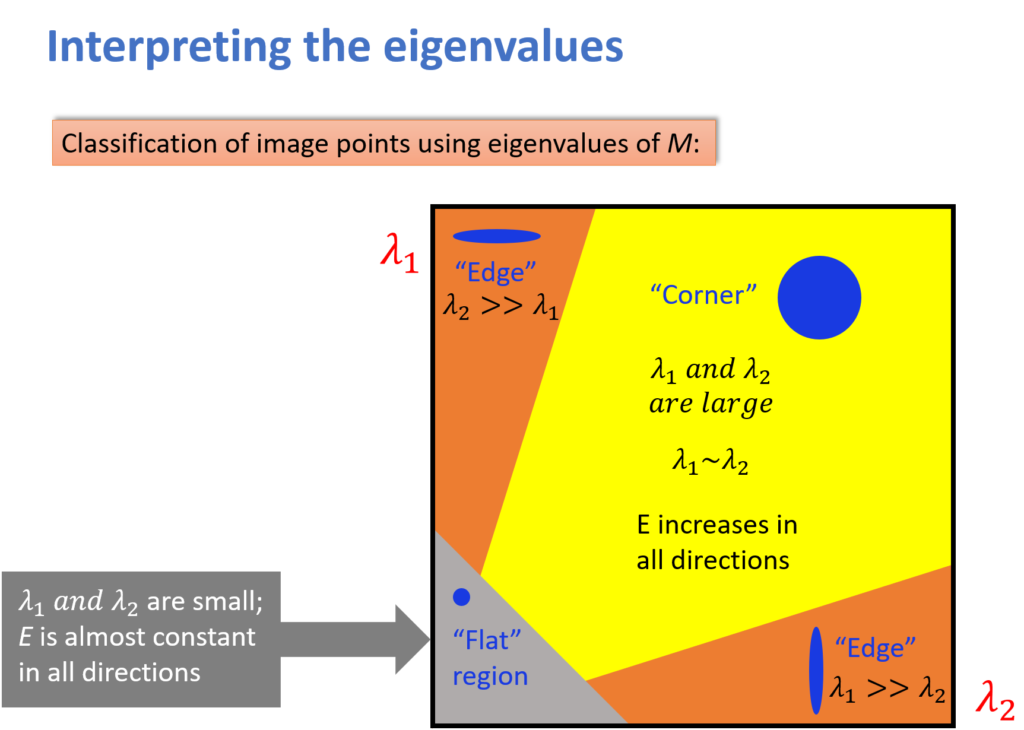
\includegraphics{wiki/eigen.png}
\caption{eigen value interpretation}
\end{figure}

    \begin{Verbatim}[commandchars=\\\{\}]
{\color{incolor}In [{\color{incolor}57}]:} \PY{k}{def} \PY{n+nf}{get\PYZus{}theta\PYZus{}conf}\PY{p}{(}\PY{n}{eigvals}\PY{p}{,} \PY{n}{eigvecs}\PY{p}{,} \PY{n}{angles}\PY{p}{)}\PY{p}{:}
             \PY{l+s+sd}{\PYZdq{}\PYZdq{}\PYZdq{}}
         \PY{l+s+sd}{    Computes theta(direction) and confidence degrees of lines using eigen matrices}
         \PY{l+s+sd}{    }
         \PY{l+s+sd}{    :param eignvecs: Eigen vectors of covariance matrix of each direction}
         \PY{l+s+sd}{    :param eignvals: Eigen values of covariance matrix of each direction}
         \PY{l+s+sd}{    :param angles: possible angles of given direction matrix}
         \PY{l+s+sd}{    \PYZdq{}\PYZdq{}\PYZdq{}}
         
             \PY{n}{thetas} \PY{o}{=} \PY{p}{\PYZob{}}\PY{p}{\PYZcb{}}
             \PY{n}{confidences} \PY{o}{=} \PY{p}{\PYZob{}}\PY{p}{\PYZcb{}}
         
             \PY{k}{for} \PY{n}{a} \PY{o+ow}{in} \PY{n}{ANGLES}\PY{p}{:}
                 \PY{n}{n\PYZus{}components} \PY{o}{=} \PY{n}{eigvals}\PY{p}{[}\PY{n+nb}{str}\PY{p}{(}\PY{n}{a}\PY{p}{)}\PY{p}{]}\PY{o}{.}\PY{n}{shape}\PY{p}{[}\PY{l+m+mi}{0}\PY{p}{]}
                 \PY{n}{thetas\PYZus{}comp} \PY{o}{=} \PY{n}{np}\PY{o}{.}\PY{n}{zeros}\PY{p}{(}\PY{p}{(}\PY{n}{n\PYZus{}components}\PY{p}{,} \PY{l+m+mi}{1}\PY{p}{)}\PY{p}{)}
                 \PY{n}{confidences\PYZus{}comp} \PY{o}{=} \PY{n}{np}\PY{o}{.}\PY{n}{zeros}\PY{p}{(}\PY{p}{(}\PY{n}{n\PYZus{}components}\PY{p}{,} \PY{l+m+mi}{1}\PY{p}{)}\PY{p}{)}
                 \PY{k}{for} \PY{n}{i} \PY{o+ow}{in} \PY{n+nb}{range}\PY{p}{(}\PY{n}{n\PYZus{}components}\PY{p}{)}\PY{p}{:}
                     \PY{n}{thetas\PYZus{}comp}\PY{p}{[}\PY{n}{i}\PY{p}{,}\PY{p}{:}\PY{p}{]} \PY{o}{=} \PY{n}{np}\PY{o}{.}\PY{n}{rad2deg}\PY{p}{(}\PY{n}{np}\PY{o}{.}\PY{n}{arctan2}\PY{p}{(}\PY{n}{eigvecs}\PY{p}{[}\PY{n+nb}{str}\PY{p}{(}\PY{n}{a}\PY{p}{)}\PY{p}{]}\PY{p}{[}\PY{n}{i}\PY{p}{]}\PY{p}{[}\PY{l+m+mi}{1}\PY{p}{,}\PY{l+m+mi}{1}\PY{p}{]}\PY{p}{,} \PY{n}{eigvecs}\PY{p}{[}\PY{n+nb}{str}\PY{p}{(}\PY{n}{a}\PY{p}{)}\PY{p}{]}\PY{p}{[}\PY{n}{i}\PY{p}{]}\PY{p}{[}\PY{l+m+mi}{0}\PY{p}{,}\PY{l+m+mi}{1}\PY{p}{]}\PY{p}{)}\PY{p}{)}
                     \PY{n}{confidences\PYZus{}comp}\PY{p}{[}\PY{n}{i}\PY{p}{,}\PY{p}{:}\PY{p}{]} \PY{o}{=} \PY{n}{eigvals}\PY{p}{[}\PY{n+nb}{str}\PY{p}{(}\PY{n}{a}\PY{p}{)}\PY{p}{]}\PY{p}{[}\PY{n}{i}\PY{p}{]}\PY{p}{[}\PY{l+m+mi}{1}\PY{p}{]} \PY{o}{/} \PY{p}{(}\PY{n}{eigvals}\PY{p}{[}\PY{n+nb}{str}\PY{p}{(}\PY{n}{a}\PY{p}{)}\PY{p}{]}\PY{p}{[}\PY{n}{i}\PY{p}{]}\PY{p}{[}\PY{l+m+mi}{0}\PY{p}{]}\PY{o}{+}\PY{l+m+mf}{1e\PYZhy{}10}\PY{p}{)}
                 \PY{n}{thetas}\PY{p}{[}\PY{n+nb}{str}\PY{p}{(}\PY{n}{a}\PY{p}{)}\PY{p}{]} \PY{o}{=} \PY{n}{thetas\PYZus{}comp}
                 \PY{n}{confidences}\PY{p}{[}\PY{n+nb}{str}\PY{p}{(}\PY{n}{a}\PY{p}{)}\PY{p}{]} \PY{o}{=} \PY{n}{confidences\PYZus{}comp}
             \PY{k}{return} \PY{n}{thetas}\PY{p}{,} \PY{n}{confidences}
         
         \PY{n}{thetas}\PY{p}{,} \PY{n}{confidences} \PY{o}{=} \PY{n}{get\PYZus{}theta\PYZus{}conf}\PY{p}{(}\PY{n}{eigvals}\PY{p}{,} \PY{n}{eigvecs}\PY{p}{,} \PY{n}{ANGLES}\PY{p}{)}
         \PY{n+nb}{print}\PY{p}{(}\PY{n}{thetas}\PY{p}{[}\PY{l+s+s1}{\PYZsq{}}\PY{l+s+s1}{90}\PY{l+s+s1}{\PYZsq{}}\PY{p}{]}\PY{p}{[}\PY{l+m+mi}{0}\PY{p}{]}\PY{p}{)}
         \PY{n+nb}{print}\PY{p}{(}\PY{n}{confidences}\PY{p}{[}\PY{l+s+s1}{\PYZsq{}}\PY{l+s+s1}{90}\PY{l+s+s1}{\PYZsq{}}\PY{p}{]}\PY{p}{[}\PY{l+m+mi}{0}\PY{p}{]}\PY{p}{)}
\end{Verbatim}


    \begin{Verbatim}[commandchars=\\\{\}]
89.9999999999
32.999999987

    \end{Verbatim}

    \hypertarget{d-threshold}{%
\subsubsection{2.D Threshold}\label{d-threshold}}

    \begin{Verbatim}[commandchars=\\\{\}]
{\color{incolor}In [{\color{incolor}58}]:} \PY{n}{threshold} \PY{o}{=} \PY{l+m+mi}{5}
         
         \PY{k}{def} \PY{n+nf}{threshold\PYZus{}conf}\PY{p}{(}\PY{n}{confidences}\PY{p}{,} \PY{n}{threshold}\PY{p}{,} \PY{n}{angles}\PY{p}{)}\PY{p}{:}
             \PY{l+s+sd}{\PYZdq{}\PYZdq{}\PYZdq{}}
         \PY{l+s+sd}{    Thresholds each confidence of each direction for all directions in angles}
         \PY{l+s+sd}{    }
         \PY{l+s+sd}{    :param confidences: confidence degrees of lines using eigen matrices}
         \PY{l+s+sd}{    :param threshold: threshold value for confidence score}
         \PY{l+s+sd}{    :param angle: possible angles of given direction matrix}
         \PY{l+s+sd}{    \PYZdq{}\PYZdq{}\PYZdq{}}
         
             \PY{n}{strong\PYZus{}confs} \PY{o}{=} \PY{p}{\PYZob{}}\PY{p}{\PYZcb{}}
             \PY{k}{for} \PY{n}{a} \PY{o+ow}{in} \PY{n}{ANGLES}\PY{p}{:}
                 \PY{n}{n\PYZus{}components} \PY{o}{=} \PY{n}{confidences}\PY{p}{[}\PY{n+nb}{str}\PY{p}{(}\PY{n}{a}\PY{p}{)}\PY{p}{]}\PY{o}{.}\PY{n}{shape}\PY{p}{[}\PY{l+m+mi}{0}\PY{p}{]}
                 \PY{n}{strong\PYZus{}conf\PYZus{}comp} \PY{o}{=} \PY{n}{np}\PY{o}{.}\PY{n}{zeros}\PY{p}{(}\PY{p}{(}\PY{n}{n\PYZus{}components}\PY{p}{,} \PY{l+m+mi}{1}\PY{p}{)}\PY{p}{)}
                 \PY{k}{for} \PY{n}{i} \PY{o+ow}{in} \PY{n+nb}{range}\PY{p}{(}\PY{n}{n\PYZus{}components}\PY{p}{)}\PY{p}{:}
                     \PY{n}{strong\PYZus{}conf\PYZus{}comp}\PY{p}{[}\PY{n}{i}\PY{p}{,}\PY{p}{:}\PY{p}{]} \PY{o}{=} \PY{l+m+mi}{1} \PY{k}{if} \PY{n}{confidences}\PY{p}{[}\PY{n+nb}{str}\PY{p}{(}\PY{n}{a}\PY{p}{)}\PY{p}{]}\PY{p}{[}\PY{n}{i}\PY{p}{]} \PY{o}{\PYZgt{}} \PY{n}{threshold} \PY{k}{else} \PY{l+m+mi}{0}
                 \PY{n}{strong\PYZus{}confs}\PY{p}{[}\PY{n+nb}{str}\PY{p}{(}\PY{n}{a}\PY{p}{)}\PY{p}{]} \PY{o}{=} \PY{n}{strong\PYZus{}conf\PYZus{}comp}
             \PY{k}{return} \PY{n}{strong\PYZus{}confs}
         
         \PY{n}{strong\PYZus{}confs} \PY{o}{=} \PY{n}{threshold\PYZus{}conf}\PY{p}{(}\PY{n}{confidences}\PY{p}{,} \PY{n}{threshold}\PY{p}{,} \PY{n}{ANGLES}\PY{p}{)}
         \PY{n}{strong\PYZus{}confs}
\end{Verbatim}


\begin{Verbatim}[commandchars=\\\{\}]
{\color{outcolor}Out[{\color{outcolor}58}]:} \{'0': False, '45': False, '90': True, '135': False\}
\end{Verbatim}
            
    \hypertarget{e-test}{%
\subsubsection{2.E Test}\label{e-test}}

    \begin{Verbatim}[commandchars=\\\{\}]
{\color{incolor}In [{\color{incolor}59}]:} \PY{n}{image} \PY{o}{=} \PY{n}{cv2}\PY{o}{.}\PY{n}{imread}\PY{p}{(}\PY{l+s+s1}{\PYZsq{}}\PY{l+s+s1}{images/cameraman.jpg}\PY{l+s+s1}{\PYZsq{}}\PY{p}{,} \PY{l+m+mi}{0}\PY{p}{)}\PY{o}{.}\PY{n}{astype}\PY{p}{(}\PY{n+nb}{float}\PY{p}{)}
         \PY{n}{image\PYZus{}blurred} \PY{o}{=} \PY{n}{GaussianNoise}\PY{p}{(}\PY{p}{)}\PY{p}{(}\PY{n}{image}\PY{p}{)}
         \PY{n}{image\PYZus{}grad}\PY{p}{,} \PY{n}{image\PYZus{}theta} \PY{o}{=} \PY{n}{GradientIntensity}\PY{p}{(}\PY{p}{)}\PY{p}{(}\PY{n}{image\PYZus{}blurred}\PY{p}{)}
         \PY{n}{image\PYZus{}suppressed} \PY{o}{=} \PY{n}{NonMaxSuppression}\PY{p}{(}\PY{p}{)}\PY{p}{(}\PY{n}{image\PYZus{}grad}\PY{p}{,} \PY{n}{image\PYZus{}theta}\PY{p}{)}
         \PY{n}{image\PYZus{}final} \PY{o}{=} \PY{n}{Thresholding}\PY{p}{(}\PY{p}{)}\PY{p}{(}\PY{n}{image\PYZus{}suppressed}\PY{p}{)}
         \PY{n}{image\PYZus{}final}\PY{p}{[}\PY{n}{image\PYZus{}final}\PY{o}{\PYZlt{}} \PY{l+m+mi}{1}\PY{p}{]} \PY{o}{=} \PY{l+m+mi}{0} 
         \PY{n}{image\PYZus{}final}\PY{p}{[}\PY{n}{image\PYZus{}final}\PY{o}{\PYZgt{}} \PY{l+m+mi}{1}\PY{p}{]} \PY{o}{=} \PY{l+m+mi}{255}
         \PY{n}{image\PYZus{}final} \PY{o}{=} \PY{n}{image\PYZus{}final}\PY{o}{.}\PY{n}{astype}\PY{p}{(}\PY{n}{np}\PY{o}{.}\PY{n}{uint8}\PY{p}{)}
         \PY{n}{plt}\PY{o}{.}\PY{n}{imshow}\PY{p}{(}\PY{n}{image\PYZus{}final}\PY{p}{,} \PY{n}{cmap}\PY{o}{=}\PY{l+s+s1}{\PYZsq{}}\PY{l+s+s1}{gray}\PY{l+s+s1}{\PYZsq{}}\PY{p}{)}
\end{Verbatim}


\begin{Verbatim}[commandchars=\\\{\}]
{\color{outcolor}Out[{\color{outcolor}59}]:} <matplotlib.image.AxesImage at 0x1c5e330d390>
\end{Verbatim}
            
    \begin{center}
    \adjustimage{max size={0.9\linewidth}{0.9\paperheight}}{output_33_1.png}
    \end{center}
    { \hspace*{\fill} \\}
    
    \begin{Verbatim}[commandchars=\\\{\}]
{\color{incolor}In [{\color{incolor}60}]:} \PY{k+kn}{from} \PY{n+nn}{copy} \PY{k}{import} \PY{n}{deepcopy}
         \PY{n}{image\PYZus{}} \PY{o}{=} \PY{n}{deepcopy}\PY{p}{(}\PY{n}{image\PYZus{}final}\PY{p}{)}
\end{Verbatim}


    \begin{Verbatim}[commandchars=\\\{\}]
{\color{incolor}In [{\color{incolor}121}]:} \PY{n}{directions} \PY{o}{=} \PY{n}{assign\PYZus{}direction}\PY{p}{(}\PY{n}{image\PYZus{}theta}\PY{p}{)}
          \PY{n}{directions} \PY{o}{=} \PY{n}{np}\PY{o}{.}\PY{n}{multiply}\PY{p}{(}\PY{n}{directions}\PY{p}{,} \PY{n}{image\PYZus{}final}\PY{o}{==}\PY{l+m+mi}{255}\PY{p}{)}  \PY{c+c1}{\PYZsh{} mask out non\PYZhy{}edge directions}
          \PY{n}{plt}\PY{o}{.}\PY{n}{imshow}\PY{p}{(}\PY{n}{directions}\PY{p}{,} \PY{n}{cmap}\PY{o}{=}\PY{l+s+s1}{\PYZsq{}}\PY{l+s+s1}{gray}\PY{l+s+s1}{\PYZsq{}}\PY{p}{)}
\end{Verbatim}


\begin{Verbatim}[commandchars=\\\{\}]
{\color{outcolor}Out[{\color{outcolor}121}]:} <matplotlib.image.AxesImage at 0x1c5e4afd240>
\end{Verbatim}
            
    \begin{center}
    \adjustimage{max size={0.9\linewidth}{0.9\paperheight}}{output_35_1.png}
    \end{center}
    { \hspace*{\fill} \\}
    
    \begin{Verbatim}[commandchars=\\\{\}]
{\color{incolor}In [{\color{incolor}85}]:} \PY{n}{ANGLES} \PY{o}{=} \PY{p}{[}\PY{l+m+mi}{0}\PY{p}{,} \PY{l+m+mi}{45}\PY{p}{,} \PY{l+m+mi}{90}\PY{p}{,} \PY{l+m+mi}{135}\PY{p}{]}
         \PY{n}{connected\PYZus{}components} \PY{o}{=} \PY{n}{get\PYZus{}connected\PYZus{}components}\PY{p}{(}\PY{n}{directions}\PY{p}{,} \PY{n}{ANGLES}\PY{p}{)}
         
         \PY{n}{plt}\PY{o}{.}\PY{n}{figure}\PY{p}{(}\PY{n}{figsize}\PY{o}{=}\PY{p}{(}\PY{l+m+mi}{20}\PY{p}{,} \PY{l+m+mi}{20}\PY{p}{)}\PY{p}{)}
         
         \PY{k}{for} \PY{n}{i}\PY{p}{,}\PY{n}{a} \PY{o+ow}{in} \PY{n+nb}{enumerate}\PY{p}{(}\PY{n}{ANGLES}\PY{p}{)}\PY{p}{:}
             \PY{n}{plt}\PY{o}{.}\PY{n}{subplot}\PY{p}{(}\PY{l+m+mi}{1}\PY{p}{,}\PY{l+m+mi}{4}\PY{p}{,} \PY{n+nb}{int}\PY{p}{(}\PY{n}{i}\PY{o}{+}\PY{l+m+mi}{1}\PY{p}{)}\PY{p}{)}
             \PY{n}{plt}\PY{o}{.}\PY{n}{imshow}\PY{p}{(}\PY{n}{connected\PYZus{}components}\PY{p}{[}\PY{n+nb}{str}\PY{p}{(}\PY{n}{a}\PY{p}{)}\PY{p}{]}\PY{p}{,} \PY{n}{cmap}\PY{o}{=}\PY{l+s+s1}{\PYZsq{}}\PY{l+s+s1}{gray}\PY{l+s+s1}{\PYZsq{}}\PY{p}{)}
             \PY{n}{plt}\PY{o}{.}\PY{n}{title}\PY{p}{(}\PY{l+s+s1}{\PYZsq{}}\PY{l+s+s1}{\PYZsh{}comp}\PY{l+s+s1}{\PYZsq{}}\PY{o}{+}\PY{n+nb}{str}\PY{p}{(}\PY{n}{np}\PY{o}{.}\PY{n}{max}\PY{p}{(}\PY{n}{connected\PYZus{}components}\PY{p}{[}\PY{n+nb}{str}\PY{p}{(}\PY{n}{a}\PY{p}{)}\PY{p}{]}\PY{p}{)}\PY{p}{)}\PY{p}{)}
\end{Verbatim}


    \begin{center}
    \adjustimage{max size={0.9\linewidth}{0.9\paperheight}}{output_36_0.png}
    \end{center}
    { \hspace*{\fill} \\}
    
    \begin{Verbatim}[commandchars=\\\{\}]
{\color{incolor}In [{\color{incolor}123}]:} \PY{n}{cov\PYZus{}matrices} \PY{o}{=} \PY{n}{get\PYZus{}cov\PYZus{}matrices}\PY{p}{(}\PY{n}{connected\PYZus{}components}\PY{p}{,} \PY{n}{ANGLES}\PY{p}{)}
          \PY{n}{eigvals}\PY{p}{,} \PY{n}{eigvecs} \PY{o}{=} \PY{n}{get\PYZus{}eigens}\PY{p}{(}\PY{n}{cov\PYZus{}matrices}\PY{p}{,} \PY{n}{ANGLES}\PY{p}{)}
\end{Verbatim}


    \begin{Verbatim}[commandchars=\\\{\}]
{\color{incolor}In [{\color{incolor}125}]:} \PY{n}{thetas}\PY{p}{,} \PY{n}{confidences} \PY{o}{=} \PY{n}{get\PYZus{}theta\PYZus{}conf}\PY{p}{(}\PY{n}{eigvals}\PY{p}{,} \PY{n}{eigvecs}\PY{p}{,} \PY{n}{ANGLES}\PY{p}{)}
          
          \PY{n+nb}{print}\PY{p}{(}\PY{l+s+s1}{\PYZsq{}}\PY{l+s+s1}{thetas:}\PY{l+s+s1}{\PYZsq{}}\PY{p}{)}
          \PY{k}{for} \PY{n}{a} \PY{o+ow}{in} \PY{n}{ANGLES}\PY{p}{:}
              \PY{n+nb}{print}\PY{p}{(}\PY{n}{thetas}\PY{p}{[}\PY{n+nb}{str}\PY{p}{(}\PY{n}{a}\PY{p}{)}\PY{p}{]}\PY{o}{.}\PY{n}{shape}\PY{p}{)}
          \PY{n+nb}{print}\PY{p}{(}\PY{l+s+s1}{\PYZsq{}}\PY{l+s+se}{\PYZbs{}n}\PY{l+s+se}{\PYZbs{}n}\PY{l+s+s1}{confidences:}\PY{l+s+s1}{\PYZsq{}}\PY{p}{)}
          \PY{k}{for} \PY{n}{a} \PY{o+ow}{in} \PY{n}{ANGLES}\PY{p}{:}
              \PY{n+nb}{print}\PY{p}{(}\PY{n}{confidences}\PY{p}{[}\PY{n+nb}{str}\PY{p}{(}\PY{n}{a}\PY{p}{)}\PY{p}{]}\PY{o}{.}\PY{n}{shape}\PY{p}{)}
\end{Verbatim}


    \begin{Verbatim}[commandchars=\\\{\}]
thetas:
(1, 1)
(163, 1)
(141, 1)
(137, 1)


confidences:
(1, 1)
(163, 1)
(141, 1)
(137, 1)

    \end{Verbatim}

    \begin{Verbatim}[commandchars=\\\{\}]
{\color{incolor}In [{\color{incolor}255}]:} \PY{n}{threshold} \PY{o}{=} \PY{n}{np}\PY{o}{.}\PY{n}{mean}\PY{p}{(}\PY{p}{[}\PY{n}{np}\PY{o}{.}\PY{n}{mean}\PY{p}{(}\PY{n}{confidences}\PY{p}{[}\PY{n+nb}{str}\PY{p}{(}\PY{n}{a}\PY{p}{)}\PY{p}{]}\PY{p}{)} \PY{k}{for} \PY{n}{a} \PY{o+ow}{in} \PY{n}{ANGLES}\PY{p}{]}\PY{p}{)}\PY{o}{/}\PY{l+m+mi}{10}
          \PY{n}{strong\PYZus{}confs} \PY{o}{=} \PY{n}{threshold\PYZus{}conf}\PY{p}{(}\PY{n}{confidences}\PY{p}{,} \PY{n}{threshold}\PY{p}{,} \PY{n}{ANGLES}\PY{p}{)}
          
          \PY{k}{for} \PY{n}{a} \PY{o+ow}{in} \PY{n}{ANGLES}\PY{p}{:}
              \PY{n+nb}{print}\PY{p}{(}\PY{l+s+s1}{\PYZsq{}}\PY{l+s+s1}{\PYZsh{} of connected components with enough conf for }\PY{l+s+si}{\PYZob{}\PYZcb{}}\PY{l+s+s1}{ degree: }\PY{l+s+si}{\PYZob{}\PYZcb{}}\PY{l+s+s1}{\PYZsq{}}\PY{o}{.}\PY{n}{format}\PY{p}{(}\PY{n}{a}\PY{p}{,} \PY{n+nb}{int}\PY{p}{(}\PY{n}{np}\PY{o}{.}\PY{n}{sum}\PY{p}{(}\PY{n}{strong\PYZus{}confs}\PY{p}{[}\PY{n+nb}{str}\PY{p}{(}\PY{n}{a}\PY{p}{)}\PY{p}{]}\PY{p}{)}\PY{p}{)}\PY{p}{)}\PY{p}{)}
\end{Verbatim}


    \begin{Verbatim}[commandchars=\\\{\}]
\# of connected components with enough conf for 0 degree: 0
\# of connected components with enough conf for 45 degree: 8
\# of connected components with enough conf for 90 degree: 61
\# of connected components with enough conf for 135 degree: 4

    \end{Verbatim}

    \begin{Verbatim}[commandchars=\\\{\}]
{\color{incolor}In [{\color{incolor}256}]:} \PY{n}{connected\PYZus{}components}\PY{p}{[}\PY{l+s+s1}{\PYZsq{}}\PY{l+s+s1}{90}\PY{l+s+s1}{\PYZsq{}}\PY{p}{]}\PY{o}{.}\PY{n}{shape}
\end{Verbatim}


\begin{Verbatim}[commandchars=\\\{\}]
{\color{outcolor}Out[{\color{outcolor}256}]:} (256, 256)
\end{Verbatim}
            
    \begin{Verbatim}[commandchars=\\\{\}]
{\color{incolor}In [{\color{incolor}257}]:} \PY{n}{strong\PYZus{}confs}\PY{p}{[}\PY{l+s+s1}{\PYZsq{}}\PY{l+s+s1}{90}\PY{l+s+s1}{\PYZsq{}}\PY{p}{]}\PY{o}{.}\PY{n}{nonzero}\PY{p}{(}\PY{p}{)}\PY{p}{[}\PY{l+m+mi}{0}\PY{p}{]}
\end{Verbatim}


\begin{Verbatim}[commandchars=\\\{\}]
{\color{outcolor}Out[{\color{outcolor}257}]:} array([  1,   2,   3,   4,   5,   6,   7,  10,  11,  15,  19,  20,  21,
                  22,  25,  27,  28,  29,  31,  34,  36,  37,  38,  39,  43,  46,
                  47,  48,  50,  51,  52,  53,  55,  57,  59,  61,  68,  75,  76,
                  77,  78,  81,  82,  91,  92,  93,  94,  95,  96,  97, 100, 103,
                 108, 112, 116, 120, 123, 124, 125, 127, 135], dtype=int64)
\end{Verbatim}
            
    \begin{Verbatim}[commandchars=\\\{\}]
{\color{incolor}In [{\color{incolor}303}]:} \PY{n}{plt}\PY{o}{.}\PY{n}{imshow}\PY{p}{(}\PY{n}{connected\PYZus{}components}\PY{p}{[}\PY{l+s+s1}{\PYZsq{}}\PY{l+s+s1}{90}\PY{l+s+s1}{\PYZsq{}}\PY{p}{]}\PY{o}{==}\PY{l+m+mi}{46}\PY{p}{,} \PY{n}{cmap}\PY{o}{=}\PY{l+s+s1}{\PYZsq{}}\PY{l+s+s1}{gray}\PY{l+s+s1}{\PYZsq{}}\PY{p}{)}
\end{Verbatim}


\begin{Verbatim}[commandchars=\\\{\}]
{\color{outcolor}Out[{\color{outcolor}303}]:} <matplotlib.image.AxesImage at 0x1c5e96e4e10>
\end{Verbatim}
            
    \begin{center}
    \adjustimage{max size={0.9\linewidth}{0.9\paperheight}}{output_42_1.png}
    \end{center}
    { \hspace*{\fill} \\}
    
    \begin{Verbatim}[commandchars=\\\{\}]
{\color{incolor}In [{\color{incolor}305}]:} \PY{n}{plt}\PY{o}{.}\PY{n}{imshow}\PY{p}{(}\PY{n}{connected\PYZus{}components}\PY{p}{[}\PY{l+s+s1}{\PYZsq{}}\PY{l+s+s1}{45}\PY{l+s+s1}{\PYZsq{}}\PY{p}{]}\PY{o}{==}\PY{l+m+mi}{51}\PY{p}{,} \PY{n}{cmap}\PY{o}{=}\PY{l+s+s1}{\PYZsq{}}\PY{l+s+s1}{gray}\PY{l+s+s1}{\PYZsq{}}\PY{p}{)}
\end{Verbatim}


\begin{Verbatim}[commandchars=\\\{\}]
{\color{outcolor}Out[{\color{outcolor}305}]:} <matplotlib.image.AxesImage at 0x1c5e9796f28>
\end{Verbatim}
            
    \begin{center}
    \adjustimage{max size={0.9\linewidth}{0.9\paperheight}}{output_43_1.png}
    \end{center}
    { \hspace*{\fill} \\}
    

    % Add a bibliography block to the postdoc
    
    
    
    \end{document}
